\documentclass[a4paper, table]{article}

\usepackage{xcolor}
\usepackage{amssymb}
\usepackage[a4paper]{geometry}
\usepackage[T1]{fontenc}
\usepackage[utf8]{inputenc}
\usepackage{graphicx}
\usepackage{todonotes}
\usepackage{hyperref}
\usepackage{longtable}
\usepackage{times}
\usepackage{pdflscape}
\usepackage[style=verbose-ibid,backend=bibtex]{biblatex}
\usepackage{listings}

\definecolor{dkgreen}{rgb}{0,0.6,0}
\definecolor{gray}{rgb}{0.5,0.5,0.5}
\definecolor{mauve}{rgb}{0.58,0,0.82}

\lstset
{
    frame=none,
    basicstyle={\small\ttfamily},
    commentstyle=\color{dkgreen},
    stringstyle=\color{mauve},
    numbers=none, %Nummerierung
    numberstyle=\tiny\color{gray},
    showstringspaces=false,
    breaklines=true,
    aboveskip=3mm,
    belowskip=3mm,
    columns=flexible,
    breakatwhitespace=true
}

\lstdefinelanguage{csharp}
{
    language=[Sharp]C,
    keywordstyle=\color{blue},
    tabsize=3,
    morekeywords={partial, var, value, get, set}
}

\lstdefinelanguage{json}
{
    stepnumber=1,
    numbersep=8pt,
    string=[s]{"}{"},
    comment=[l]{:\ "},
    morecomment=[l]{:"},
    literate=
        *{0}{{{\color{numb}0}}}{1}
         {1}{{{\color{numb}1}}}{1}
         {2}{{{\color{numb}2}}}{1}
         {3}{{{\color{numb}3}}}{1}
         {4}{{{\color{numb}4}}}{1}
         {5}{{{\color{numb}5}}}{1}
         {6}{{{\color{numb}6}}}{1}
         {7}{{{\color{numb}7}}}{1}
         {8}{{{\color{numb}8}}}{1}
         {9}{{{\color{numb}9}}}{1}
}

\lstdefinestyle{XML}
{
    morestring=[b]",
    moredelim=[s][\bfseries\color{green}]{<}{\ },
    moredelim=[s][\bfseries\color{green}]{</}{>},
    moredelim=[l][\bfseries\color{green}]{/>},
    moredelim=[l][\bfseries\color{green}]{>},
    morecomment=[s]{<?}{?>},
    morecomment=[s]{<!--}{-->},
    identifierstyle=\color{blue}
}

\hypersetup{
    colorlinks=true,
    linkcolor=darkgray,
    filecolor=magenta,
    urlcolor=blue
}
\urlstyle{same}

\bibliography{wipro-main-doc}
\graphicspath{ {images/} }

\newcommand{\tabitem}{~~\llap{\textbullet}~~}
\newcommand{\rot}{\rotatebox{90}}

% Set name of image label
\renewcommand{\figurename}{Abbildung}

\title{
    {Wirtschaftsprojekt} \\
    \vspace{10mm}
    { Herbstsemester 2022 } \\
    \vspace{10mm}
    % https://commons.wikimedia.org/wiki/File:HSLU_2022_logo.svg
    {
\includegraphics[width=75mm]{img/hsluLogo2022.png}}
}

\author{Yannis Kr\"amer und Nicolas Wiedmer}
% TODO: Update date
\date{21.12.2022}

\begin{document}

\maketitle

\newpage

\noindent
\fontsize{12}{14}
\textbf{Wirtschaftsprojekt an der Hochschule Luzern -- Informatik} \\ \vspace*{0.6cm}

\fontsize{10.95}{12}
\noindent
\textbf{Titel:} STAIR Discord Bot \\ \vspace*{0.2cm}

\noindent
\textbf{Studentin/Student:} Yannis Kr\"amer \newline \newline
\textbf{Studentin/Student:} Nicolas Wiedmer \newline \newline
\textbf{Studiengang:} BSc Informatik oder Wirtschaftsinformatik  \newline \newline
\textbf{Jahr:} 2022 \newline \newline
\textbf{Betreuungsperson:} Markus Waldmann \newline \newline
\textbf{Expertin/Experte:} \newline \newline
\textbf{Auftraggeberin/Auftraggeber:} STAIR (Martin Steiger \& Estefania Otero)\newline \newline \newline
\textbf{Codierung / Klassifizierung der Arbeit:}\\
$\boxtimes$ \"Offentlich
$\square$ Vertraulich


%%% you can use \boxtimes for filling a cross inside the square
%%% e.g., $\boxtimes$ A: Einsicht 	(Normalfall)


\paragraph{\textbf{Eidesstattliche Erkl\"arung}}
Ich erkl\"are hiermit, dass ich/wir die vorliegende Arbeit selbst\"andig und ohne unerlaubte fremde Hilfe angefertigt haben, alle verwendeten Quellen, Literatur und andere Hilfsmittel angegeben haben, w\"ortlich oder inhaltlich entnommene Stellen als solche kenntlich gemacht haben, das Vertraulichkeitsinteresse des Auftraggebers wahren und die Urheberrechtsbestimmungen der Hochschule Luzern respektieren werden. \newline \newline
Ort / Datum, Unterschrift	\underline{\hspace*{8cm}} \newline \newline
Ort / Datum, Unterschrift	\underline{\hspace*{8cm}} \newline \newline \newline
\textbf{Ausschliesslich bei Abgabe in gedruckter Form: \\
Eingangsvisum durch das Sekretariat auszuf\"ullen}\newline \newline
Rotkreuz, den	\underline{\hspace*{4cm}}	\hspace*{1cm} Visum:	\underline{\hspace*{4cm}}

\normalfont
\newpage
\section*{I{\hspace*{1cm}}Abstract}
\todo{schreiben}

\newpage

\tableofcontents

\newpage

\section{Problem, Fragestellung, Vision}
Der Studentenverein STAIR des Departemnts Informatik der Hochschule Luzern stellt über die Plattform Discord einen Server zur Verfügung.
Über diesen können sich Studenten über das Studium oder spezifische Module austauschen.\\
Auf dem Server laufen zwei Bots, welche sich um die Authentifikation der Studenten, sowie um die Einschreibung in die verschiedenen Modul-Channels kümmern.
Der Bot zur Authentifikation funktioniert einwandfrei, aber beim Bot zur Moduleinschreibung kommt es immer wieder zu Problemen.
Da dieser extern auf einer Plattform namens Nadeko erstellt wurde, kann nicht genau gesagt werden, wieso diese Probleme auftreten.\\
Des Weiteren gibt es Unklarheiten bei den Studenten zur Benutzung dieser Bots.
Auch die Aufteilung der Modul-Channels, in verschiedene Kategorien, ist nicht benutzerfreundlich gestaltet.
In einer neuen Version, sollen die Probleme beseitigt und die Unklarheiten bei den Studenten geklärt werden.\\\\
In diesem Projekt soll eine Lösung entwickelt werden, die den Discord Administratoren von STAIR eine Unterstützung und Mehrwert beitet.
Die Lösung soll für STAIR und Studenten verständlich sein und einfach eingesetzt werden können.\\\\
Das Ziel der Arbeit ist es, die vorher beschriebenen zwei Bots zusammenzuführen und damit eine einheitliche Platform zu haben, über welchen Bot Commands verwaltet werden.
Des weiteren soll eine Datenbank eingeführt werden, die Studenten und Ihre Discord Accounts verbindet.
Dies erleichtert die Authentifikation und die Verwaltung der Modul-Channels.
Die Daten bieten auch einen statistischen Mehrwert für die STAIR Mitglieder, da ein besser Einblick gewährt wird, wer den Discord Server nutzt.
Dies kann für Marketingzwecke sowie Event-Plannung verwendet werden.\\
Auch soll der Einsatz von einer automatischen Fehlererkennung dazu beitragen, das Probleme beim Bot schnell an die Administartoren von STAIR weitergeleitet werden.
So können lange Unsicherheiten und Probleme schneller behoben werden.
Der Einsatz einer neuen Logging Library soll die Nachvollziehbarkeit der Software sicherstellen.
Diese Einträge sollen den Administratoren bei allfälligen Fehlersuchen unterstützen.\\\\ 

\newpage
\section{Stand der Technik}\label{state-of-the-art}
Als ersten Schritt soll der heutige Stand der Technik im Bereich Spach- und Text-Messaging überprüft werden.
Dabei soll aufgezeigt werden, welche mögliche Plattformen es auf dem Markt gibt, und ob diese eine mögliche Alternative zum Discord Server sind.

\subsection{Sprach- und Text-Messenger}
Die folgenden Platform sind die am weitest verbreiteten auf dem Markt, wenn es um Discord Alternativen und Sprach Chats im allgemeinen geht. \autocite{noauthor_discord-alternativen_nodate}

\subsubsection*{Slack}
Slack ist eine sehr ähnliche Alternative zu Discord, richtet sich jedoch mehr an Unternehmen als an Communities.
Dies ist auch gut auf der Homepage des jeweiligen Unternehmens zu erkennen.
So erwähnt Discord zum Beispiel: "\textit{STELL DIR EINEN ORT VOR, …
… an dem du Teil eines Schulklubs, einer Gaming-Gruppe oder einer weltweiten Kunst-Community sein kannst. Ein Ort, an dem du einfach Zeit mit Freunden verbringen kannst. Ein Ort, an dem es leicht ist, sich jederzeit zu treffen und zu unterhalten.}" \autocite{noauthor_discord_nodate}
wo hingegen Slack folgendes schreibt: "\textit{Great teamwork starts with a digital HQ
With all your people, tools and communication in one place, you can work faster and more flexibly than ever before.}"\autocite{slack_slack_nodate}
Auch der Fokus der Anwendung liegt stärker auf dem Textchat als auf dem Sprachchat, wo sich Discord widerum mehr fokusiert.\autocite{noauthor_slack_nodate}
Da STAIR und der Discord Server auch für die Freizeit gedacht sind, macht es mehr Sinn auf ein Freizeit Tool zu setzen.

\subsubsection*{Skype}
Skype ist eine ältere und sehr verbreitete Sprachchat Lösungen mit 100 Millionen aktiven Nutzern jeden Monat. \autocite{lardinois_microsoft_2020}
Skype ist jedoch auch sehr eingeschränkt, was die Features angeht.
So sind keine echten Communities möglich und Sprachchat ist nur per Anruf möglich.
So können neue Nutzer also nicht einfach zu einem Sprachchat hinzukommen.
Richtige Communities sind ebenfalls nicht vorhanden. \autocite{mattise_discord_2022}
Diese fehlenden Features machen das Programm ungeeignet als Alternative.

\subsubsection*{TeamSpeak}

TeamSpeak macht es möglich einfach und ohne viel Rechenressourcen einen Server zum Austauschen aufzusetzen.
Der Fokus von TeamSpeak sind klar die Sprachchats.
Auch wenn Textchats möglich sind, sind diese stärker eingeschränkt und klar nicht der Fokus der Anwendung.
Da Textchat nicht unwichtig ist für den Austausch den STAIR anbieten will,
ist dies wohl keine geeignete Lösung.
Ein grosser Nachteil ist, dass nur 32 aktive Nutzer kostenfrei auf einen Server kommen können.
Dies würde zu starken mehrkosten führen für STAIR.\autocite{mockel_discord_2022}

\subsubsection*{Matrix}

Matrix wurde 2019 veröffentlicht und ist eine Open Source Alternative zu Discord.
Hierbei kommt Matrix dem Discord mit der Bedienung sehr nahe.
Ein starker Fokus liegt auf der Privatsphäre der Nutzer.
So ist man unabhängig von den Entwicklern und kann den Matrix Server auf dem eigenen Server aufsetzen.
Die Software bringt jedoch auch seine Nachteile mit sich.
So ist die Verbreitung noch relativ klein und hat wenig Nutzer.
Mit 17 Millionen Nutzer\autocite{noauthor_matrixorg_nodate} hinkt Matrix noch stark an den 300 Millionen Nutzern von Discord hinten nach.\autocite{david_curry_discord_2022}
So müssten viele Studierende zuerst einen Account erstellen und sich einen Matrix aussschliesslich für den STAIR Server herunterladen. Dies wäre eine zusätzliche Hürde.
Auch wäre das betreiben des Matrix Servers umständlicher, da die Updates neu manuell installiert werden müssen anstatt dies von Discord machen zu lassen.
Auch wäre unklar, ob das Enterprise Lab eine solche Applikation zulassen würde, da dies einiges an Bandbreite kosten würde, was Discord zurzeit übernimmt für STAIR.

Der Vorteil an Matrix ist, dass jeder seinen eigenen Client wählen oder sogar entwickeln kann.\autocite{noauthor_matrix_nodate}
So sollte jeder Nutzer etwas passendes finden.
Auch ist die Privatsphäre der Studierenden geschützt, da keine Informationen nach aussen geraten wenn der Server selbst gehostet ist.

\subsubsection{Discord}
Der Online Dienst Discord ist ein Instant-Messaging und Chat Tool mit Sprach- und Videokonferenz Funktion.
Er kann online auf einer Webseite, oder mit Hilfe eines Clients lokal aufgerufen werden.
Discord unterst\"utzt alle g\"angigen Betriebssysteme und kann auch auf mobilen Endger\"aten verwendet werden.

\subsubsection*{Geschichte}
Urspr\"unglich wurde Discord f\"ur Computerspiele geschaffen, um die Kommunikation zwischen den Spielkameraden zu vereinfachen und zu verbessern.
Das Ziel war es, neben der komplexen Spielmechanik einen Chat-Messanger zu bauen, der benutzerfreundlich und effizient erweist.
2012 wurde das Unternehmen Discord Inc (damals noch Hammer \& Chisel)
als Startup gegr\"undet.\autocite{noauthor_discord_2021}
Im Jahre 2014 konnte die Unternehmung Hammer \& Chisel f\"ur die Weiterentwicklung Ihrer
Applikation auf zus\"atzliche Finanzierungsmittel, von anderen Unternehmen zur Verfügung gestellt, zurückgreifen.

2015 wurde Discord unter der Domain "discordapp.com" ver\"offentlicht.
Der Text und Sprach Messanger erfreute sich schnell grosser Beliebtheit
und geriet so in das Blickfeld grösserer Investoren wie z.B. Warner Media, die den Dienst 2016 mit rund
20 Millionen US-Dollar unterstützte. \autocite{noauthor_warner_2022} .
2018 k\"undete auch Microsoft Discord Unterst\"utzung f\"ur ihre XBox Live Nutzer an und unterst\"utzte Discord mit einer Finanzierung
von 150 Millionen US-Dollar. Bewertet wurde Discord Inc nun auf etwa 2 Milliarden US-Dollar.

Aufgrund der Covid-19 Pandemie und den steigenden Benutzerzahlen stellte sich Discord auch f\"ur andere Zielgruppen ein.
So wurde der Fokus von Videospielen weggelenkt auf einen universellen Kommunikations-und Chat Client, um es f\"ur andere Branchen,
wie das Schulwesen oder innerhalb Unternehmen, ansprechender zu machen.
Damit \"anderte das Unternehmen ihr Motto von \textit{Chat for Gamers} zu
\textit{Chat for Communities and Friends} und f\"uhrte Servervorlagen ein.

Heute hat Discord mehr als 140 Millionen monatlich aktive User, verwaltet etwa 13.5 Millionen aktive Server und
wird auf 15 Milliarden US-Dollar gewertet (Stand 2021). \autocite{david_curry_discord_2022}

\subsubsection*{Discord Einschr\"ankungen}\label{discord_einschraenkungen}
Discord hat auch einige Einschränkungen.
Diese machen sich allerdings erst bei sehr grossen Servern bemerkbar.\autocite{vultaggio_discord_2022}
\begin{itemize}
    \item Anzahl Channels: 500
    \item Anzahl Rollen: 250
    \item Anzahl Kategorien: 50
    \item Anzahl Channels pro Kategorie: 50
    \item Anzahl Mitglieder: 250'000
    \item Anzahl Freunde eines Accounts: 1000
    \item Anzahl Buchstaben für Rollen und Channels: 100
\end{itemize}

\subsubsection*{Warum Discord?}
Wie man gesehen hat, gibt es noch andere Sprach- und Text Messanger auf dem Markt.
Für dieses Projekt ist Discord verbindlich festgelegt.
STAIR kommuniziert schon lange über die Plattform und es hat sich eine grosse Community mit knapp 700 Studierenden und Exstudierenden aufgebaut.
Discord erlaubt grosse Freiheiten in der Erstellung von Servern und Channels, deren Bearbeitung und der Freigabe unter den Mitgliedern.
Da es ein kostenloser Dienst ist und diese Einstellungsmöglichkeiten hat, ist es sehr verbreitet bei jungen Leuten aller Ethnien und Gruppierungen.

\newpage
\section{Ideen und Konzepte}

Bei der Konzeptbesprechung wurde ein Entity-Relationship Diagramm ausgearbeitet.
Das Diagramm dient als Grundlage für die Design- und Architektur Entscheide der neuen Applikation.
Des Weiteren wurde ein Konzept zur allgemeinen Projektstruktur erstellt und einzelne Überlegungen zum neuen Ablauf der Authentifizierung und Modul Anmeldung.

\begin{figure}[h]
    \centering
    \includegraphics[width=1.0\textwidth]{img/Konzept_Skizze.png}
    \caption{Konzept Skizze}
    \label{fig:concept-sketch}
\end{figure}

Eine genaue Beschreibung des ER-Diagramms kann im Kapitel \nameref{entity-relationship-diagramm} gefunden werden.

\subsection{Technologien}

\subsubsection{C\# und .NET Framework}

Es wurde entschieden weiterhin mit C\# zu arbeiten.
Dies wurde auch für die bereits existierende Version verwendet.
Discord Libraries sind jedoch auch in anderen programmiersprachen verfügbar.
Discord selbst führt eine Liste zu den verfügbaren Libraries und deren unterstützten Programmiersprachen, welche von der Community entwickelt wurden.\autocite{noauthor_discord_2022-1}
Bei Besprechungen mit den Stakeholdern wurde kein Grund gesehen auf etwas anderes umzusteigen, vor allem da durch das existierende Projekte eine gewisse Machbarkeit für einen Teil der Features bereits bewiesen wurde.
Durch die neuen .NET Versionen wird es nun auch möglich den C\# Code auf andere Platformen als nur Windows zu exportieren.
Hierfür wurde früher Project Mono gebraucht oder .NET Core.
Die beiden Projekte wurden mit dem .NET Framework zusammengeführt zu der .NET 5 Version.\autocite{schwichtenberg_net_2019}
Im November 2022 ist die neue .NET 7 Version herausgekommen.
Da .NET 6 am aktuellsten war zum Startzeitpunkt des WIPRO Projektes, die .NET 6 Version eine LTS Version ist und damit länger als .NET 7 unterstützt wird und in der Praxis stärker getestet ist, wird die WIPRO mit .NET 6 zuende geführt.\autocite{noauthor_net_2022}
Zur Entwicklungszeit der alten Stan Discord Bot Version wurde noch auf .NET Framework gesetzt, weshalb der Bot auch noch nicht auf Linux lauffähig ist.
Dies war jedoch der Wunsch von STAIR für zukünftige Projekte.
Dies wird genauer im Kapitel \nameref{geplanteAenderungen} beschrieben.

\subsubsection{MySQL}

Als Datenbank wurde MySQL ausgewählt.
MSSQL hat die beste Unterstützung in C\# jedoch ist diese Kostenpflichtig.
Es gibt eine kostenfreie Version, jedoch ist diese auf 10 GB limitiert.
Dies macht die Technologie unattraktiv im Vergleich mit anderen Technologien ohne diese Einschränkungen und Kosten.\autocite{noauthor_sql_nodate}

Eine andere Version der gleichen Library, welche die MSSQL Unterstützung ermöglicht, bietet die Möglichkeit MySQL zu nützen.
Die Library heisst \textit{linq2db.MySql}.
Mit über 490'000 Downloads sollte die Stabilität für unsere Anwendung gegeben sein.\autocite{noauthor_linq2dbmysql_nodate}

\subsection{Teststrategie}\label{Teststrategie}
In diesem Projekt wird die abzugebende Software iterativ entwickelt.
Ein genauerer Beschrieb dazu ist im Kapitel \nameref{Vorgehensmodell} zu finden.
Diese Vorgehensweise erlaubt es flexibel auf neue Anforderungen zu reagieren und
während jeder Phase die Funktionalität sicher zu stellen.
\newline
Die einzelnen Komponenten innerhalb der Software werden mithilfe von Unit-Tests getestet.
Diese Tests werden nach dem AAA-Pattern "Arrange, Act, Assert" erstellt und ausgeführt. \autocite{noauthor_arrangeactassert_nodate}
Vor einem Meilenstein oder der Übergabe der Software wird die Software auch einigen manuellen Systemtests unterzogen.
\newline
Das Drehbuch für die manuellen Systemtests findet man im Kapitel \nameref{Testdrehbuch}.

\newpage
\section{Methoden}
\subsection{Literaturrecherche}
Um sich zu einem Thema zu informieren muss Literaturrecherche betrieben werden.
Für die Literaturrecherche sind 2 Methoden verfügbar. \autocite{solis_so_2021}
\begin{itemize}
    \item \textbf{Systematische Literaturrecherche}\\
    Die systematische Literaturrecherche wird benutzt, wenn man schon eine genaue Fragestellung besitzt und gezielt nach Themen sucht, um diese zu beantworten.
    \item \textbf{Unsystematische Literaturrecherche (Schneeballsystem)}\\
    Bei der unsystematischen Literaturrecherche will man sich einen Überblick über ein Thema verschaffen, bei dem noch keine Fragestellung definiert ist.
\end{itemize}
In diesem Projekt wird mit der systematischen Literaturrecherche gearbeitet.
Die Fragestellung ist definiert und es wird gezielt nach Suchbegriffen recherchiert.\\\\
Die Recherche wird in allen Teilen der Arbeit angewandt.
Beim Recherchieren des Kapitels \nameref{state-of-the-art}, der \nameref{project-management} oder in der \nameref{implementation}.
Die Recherche ist essentiell um aufgestellte Behauptungen zu untermauern und eine Lösung richtig zu implmentieren. 

\subsection{Projektführung}\label{project-management}
Um ein Projekt korrekt anzugehen und durchzuführen braucht es eine gute Projektführung.
Mit der Auswahl der Projektart und dem Vorgehensmodell, einem definierten Rahmenplan und Meilensteinen,
schafft man eine Umgebung mit der ein Projekt geplant und kontrolliert durchgeführt werden kann.
Es hilft bei vielen Beteiligten den Überblick zu bewahren und ist essentiell in der Umsetzung.

\subsubsection{Projektart}
Es gibt verschiedene Projektarten, welche je nach Vorhaben zur Anwendung kommen. Eine Projektart hilft, die erwarteten Ergebnisse zu spezifizieren
und geht auch mit der richtigen Wahl eines Vorgehensmodells daher.
\newline
Ein Projekt kann nach verschiedenen Modellen typisiert werden. Verbreitete Ansätze dabei sind:
\begin{itemize}
    \item Portfoliobezogene Projektklassifikation
    \item Externe und interne Projekte
    \item Projektarten nach Trägern
    \item Unterteilung nach Komplexität von Projektinhalt und Projektumwelt
    \item Diamond Approach
    \item oder die Erstellung eines Projektprofils\autocite{claus_husselmann_zielgerichtete_nodate} %PMRE Projekttypisierung
\end{itemize}
Auf den genaueren Beschrieb der einzelnen Modelle, wird verzichtet, da für dieses Projekt eine Vorgabe der verschiedenen Projektarten gemacht wurde.
Für zukünftige Projekte könnte man aber auf diese Projekttypisierungsmodelle zurückgreifen um sein Vorhaben genau einzustufen.
\newline

Für dieses Wirtschaftsprojekt standen folgende Projektarten zur Auswahl:
\begin{itemize}
    \item Einsatz von Standardsoftware und Services
    \item Software- und Produktentwicklung
    \item Innovationsprojekte (Projekte mit Erkenntnisgewinn, Forschungsprojekte)
    \item IT-Infrastrukturentwicklung
    \item Strukturierte Analyse und Konzeption von Systemen und Abläufen \autocite{oliver_gilbert_wipro_2022} %Wegleitung
\end{itemize}

Unsere Aufgabestellung verlangt, dass wir in einer ersten Phase, eine Analyse der bestehenden Infrastruktur und des zur Zeit laufenden Bots durchführen.
Die Analyse beruht auf der Frage, ob die zurzeit laufende Applikation, den neuen Features angepasst werden kann oder ersetzt werden muss.
In einer zweiten Phase wird evtl. ein neuer Bot in einer neuen Infrastruktur implementiert oder nur die neuen Features hinzugefügt.
In einer dritten Phase wird eine Anleitung für den zukünftigen Unterhalt des Discord-Servers und des Bots erstellt.

Aufgrund dieser Aufgabenstellung wurde die Projektart "Software- und Produktentwicklung" gewählt. Da wir eine Analyse von bestehender Software machen und
entweder bestehende Software weiterentwickeln oder eine neue erstellen.

\subsubsection{Vorgehensmodell}\label{Vorgehensmodell}
"\textit{Ein Vorgehensmodell ist eine mehr oder weniger genaue Anleitung, in welchen Schritten und durch welche Tätigkeiten das Projektziel
erreicht werden kann.}"\autocite{sarre_lufthansa-reservierung_2009}
Es beschreibt die verschiedenen Projektphasen, Meilensteine, Rollen, Aufgaben und die Arbeitsergebnisse (Artefakte) unter einheitlichen Begriffen.
Des Weiteren dient es mit verschiedenen Methoden, Techniken, Standards und kann die Übersichtlichkeit und Planbarkeit in einem Projekt stark erhöhen.
Bei Nutzung eines Vorgehensmodells ist die Wahrscheinlichkeit ein Projekt innerhalb der festgelegten Zeit, mit dem verfügbarem Budget und in einer
angemessenen Qualität fertigzustellen, insgesamt grösser. \autocite{jenny_projektmanagement_2016} %PMB Projektmanagement folie23
\newline

Man unterscheidet grundlegend zwischen klassischem und agilem Projektmanagement.
Beim klassischen Vorgehensmodellen arbeitet man meist sequentiell.
Also eine Phase folgt der anderen und baut darauf auf.
Rückkopplungen sind meistens nicht möglich und verzögern den Endtermin des Projektes.\\
Bespiele für klassische Vorgehensmodelle sind
\begin{itemize}
    \item das Wasserfallmodell, in dem die Phasen die verschiedenen Aktivitäten darstellen.
    \item das V-Modell, welches man gut für die Qualitätssicherung brauchen kann.
    \item oder Hermes, welches vor allem vom Schweizer Bund verwendet wird.
    \item etc.
\end{itemize}

Im agilen Projektmanagement arbeitet man iterativ und kann in den einzelnen Phasen immer wieder neu planen.
Dies erlaubt eine schnellere Rücksprache mit den Stakeholdern und die Einbringung neuer Ideen. \\
Beispiele für iterative Vorgehensmodelle sind
\begin{itemize}
    \item Scrum, welches den Grundstein des agilen Projektmanagement gebildet hat.
    \item SAFe steht für (Scaled Agile Framework) und erlaubt es Scrum in grossen Organisationen einzusetzen.
    \item etc. \autocite{noauthor_liste_2022}
\end{itemize}

Je nach Teamgrösse und Vorhaben eignet sich eher ein klassisches oder agiles Vorgehen.
Klassische Vorgehen werden meist bei sehr grossen Projekten eingesetzt, wie Bau- und Infrastruktur Projekten oder
innerhalb Wertschöpfungsketten. Also dort, wo es eine lange Planungsphase braucht und es keinen Sinn macht iterativ vorzugehen.
Das agile Vorgehen wird meist eher in kleineren Teams verwendet und ist vor allem in der Software-Entwicklung oder
im Marketing bekannt.
\newline

Für dieses Projekt wird SoDa (Software Development Agile) verwendet und ist ein hybrides Vorgehen,
das bedeutet ein Mix aus klassischem und agilem Vorgehen.
Es besteht auch aus verschiedenen Phasen die untereinander abgeschlossen sind,
hat aber auch einen iterativen Teil in der Konzeptions- und Realisierungsphase, bei dem man nach Scrum vorgeht.

\begin{figure}[h]
    \centering
    \includegraphics[width=1.0\textwidth]{img/SoDa.png}
    \caption{Software Development Agile}
    \label{fig:SoDa}
\end{figure}


Wie der Name schon sagt, ist es für die Software Entwicklung konzipiert und erlaubt es, die gängigen Artefakte,
welche man bei der Software Entwicklung erstellen muss, in die Projektphasen miteinzubinden.
So wird in der Initialisierungsphase der Projektauftrag, Business-Case und der Anfroderungskatalog definiert und
in der Einführungsphase können Anleitungen oder Einführungen für den operativen Einsatz erstellt werden.
Die Konzeptions- und Realisierungphase erlaubt es, die Vorteile von der agilen Vorgehensweise nach Scrum,
in der Entwicklung zu gebrauchen. Durch das Vorgehen mithilfe von Sprints können bei jedem Zyklus neue
Anforderungen erfasst und das weitere Vorgehen geplant werden. Die Sprints können beliebig lang gesetzt werden,
im Geschäftsumfeld üblich sind aber 2-Wochen.


Die verschiedenen Phasen unserer Aufgabenstellung lassen sich gut auf die verschiedenen Phasen von SoDa abbilden.
In der Initialisierungsphase wird die Analyse der jetzigen Software erstellt und das Projekt geplant.
In der Konzeptiopns- und Realisierungsphase wird in Sprints eingeteilt, die neue Software erstellt.
Und in der Einführungsphase kann die Bedienungsanleitung für den weiteren Gebrauch geschrieben werden.\\\\

\subsubsection{Rahmenplan}
Der Rahmenplan gibt ein Überblick über die ganzen Phasen des Projekts.
Die geplanten Zwischenergebnisse werden an fixen Punkten im Projekt als Meilensteine deklariert und mit konkretem Datum versehen.

\begin{figure}[h]
    \centering
    \hspace*{-2cm}
    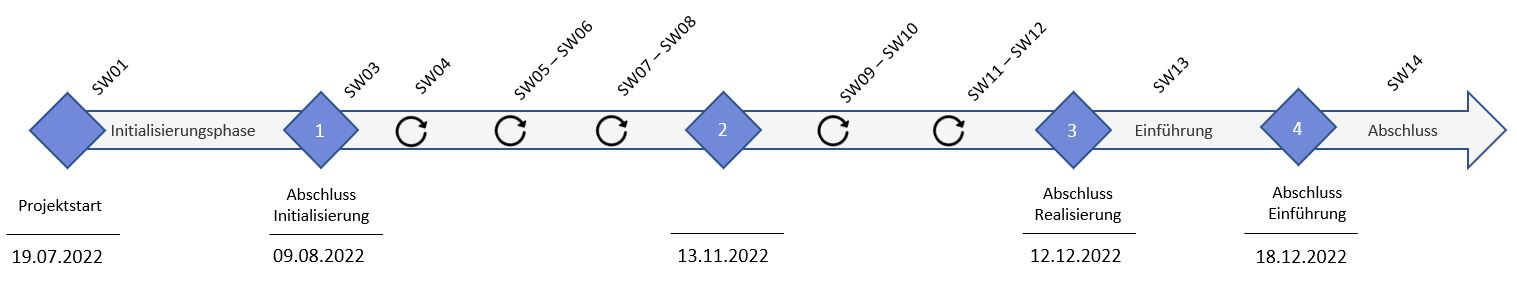
\includegraphics[width=1.3\textwidth]{img/Rahmenplan.jpg}
    \caption{Rahmenplan}
    \label{fig:Rahmenplan}
\end{figure}
Es wurde entschieden eine Intialisierungsphase von 3 Wochen zu planen, da die Analyse der bestehenden Software in dieser Phase stattfindet.
Am Schluss bleibt noch eine Woche für die Einführungsphase und das Erstellen der Anleitung.
Für die Realisierungsphase bleiben 9 Wochen Zeit, die in Sprints eingeteilt werden können.
Es verbleibt ein einwöchiger Sprint und 4 reguläre zweiwöchige Sprints.
\newpage
\subsubsection*{Meilensteine}
Meilensteine erlauben es den Projektfortschritt festzustellen,
in dem zuvor definierte Projektergebnisse (Artefakte) an einem gewissen Datum vorliegen.\\
Artefakte sind konkrete Dokumente oder Software die vorliegen muss. Zum Beispiel:
\begin{itemize}
    \item Testprotokolle
    \item Prototypen
    \item Software Releases
    \item Sprintplannungen
    \item etc.
\end{itemize}

In SoDa ist es normal, bei jedem Phasenwechsel ein Meilenstein zu definieren und in der Mitte der
Realisierungsphase noch einmal. \autocite{jenny_projektmanagement_2016} % PMB Projektplanung p23-25
Nach diesem Vorgehen erhält man 5 Meilensteine für dieses Projekt.

\begin{table}[h]
    \centering
    \begin{tabular}{|l|l|l|}
        \hline
        \rowcolor[gray]{.9} MS & Datum & Artefakte \\
        \hline
        1 & 19.09.2022 & \tabitem Aufgabenstellung \\
        \hline
        2 & 09.10.2022 & \tabitem Architekturdokument \\
         & & \tabitem Analyse \\
         & & \tabitem Testkonzept \\
         & & \tabitem Sprintplannung 1 \\
        \hline
        3 & 13.11.2022 & \tabitem Software-Release 0.5 \\
         & & \tabitem Sprintplannung 4 \\
        \hline
        4 & 12.12.2022 & \tabitem Software-Release 1.0 \\
         & & \tabitem Dokumentation Realisierung \\
        \hline
        5 & 18.12.2022 & \tabitem Bedienungsanleitung \\
        \hline
    \end{tabular}
    \caption{Meilensteine}
    \label{tab: Meilensteine}
\end{table}
\clearpage
\subsection{Risikomanagement}
Das Ziel jedes Projektes ist, eine möglichst hohe Wertschöpfung zu generieren.
Doch Wertschöpfung und Risiko stehen komplementär zueinander.
Das bedeutet, je höher die Wertschöpfung, desto höher das Risiko.
Um die Wertschöpfung möglichst hoch zu halten und die Risiken zu minimieren wird Risikomanagement betrieben.
Im Risikomanagement unterscheidet man zwischen \textbf{Produktrisiken} und \textbf{Projektrisiken}.
\newline
Produktrisiken werden direkt als Arbeitspakete im Projekt verbaut.
Dabei wird geschaut, welche Gefahren für Mensch und Umwelt während der ganzen Umsetzung und Betreibung auftreten können.
\newline
Die Projektrisiken werden im Projektmanagement behandelt.
Dabei wird geschaut, welche Probleme mich daran hindern könnten ein Projekt erfolgreich abzuschliessen.
Dies könnten sein:
\begin{itemize}
    \item technische Risiken
    \item Implementierungsrisiken
    \item wirtschaftliche, industrielle und Geschäftsrisiken
\end{itemize}
\noindent
Das Ziel des Risikomanagements ist es, Risiken frühzeitig zu erkennen und entsprechende Massnahmen zu ergreifen.
Der Prozess dabei ist folgender:
\begin{enumerate}
    \item Identifizieren
    \item Analysieren
    \item Priorisieren
    \item Massnahmen erarbeiten
    \item Überwachen \autocite[p.~8-16]{peter_sollberger_risikomanagement_2021}
\end{enumerate}
\noindent
In diesem Kapitel werden verschiedene Grundrisiken identifiziert, die während dem Projekt auftreten könnten.
Da dieses Projekt während der Umsetzungsphase iterativ läuft, kann bei den \nameref{Sprintreviews}, ein Risiko-Update durchgeführt werden.\\\\

\begin{tabular}[h]{ll}
    \textbf{Eintrittswahrscheinlichkeit} & \textbf{Schadensausmass} \\
    \tabitem Unwahrscheinlich (1) & \tabitem Gering (1) \\
    \tabitem Möglich (2) & \tabitem Mittel (2) \\
    \tabitem Wahrscheinlich (3) & \tabitem Hoch (3) \\
    \tabitem Sehr wahrscheinlich (4) & \tabitem Kritisch (4) \\
\end{tabular}
\clearpage

\begin{longtable}[ht]{|p{1em}|p{8em}|p{10em}|p{7em}|p{5em}|p{1em}|}
    \hline
    \rowcolor[gray]{.9} \rot{ID} & \rot{Risiko} & \rot{Beschreibung} & \rot{\shortstack[l]{Eintritts-\\wahrscheinlichkeit}} & \rot{Schadensausmass} & \rot{Risikoskala} \\*
    \hline
    R1 & Verbindung zwischen Bot und Discord bricht ab. &
    Die Verbindung zwischen dem Server (Discord) und dem Client (Bot) ist nicht mehr gewährleistet.
    Dies tritt ein, wenn der Bot keine Verbindung zum Internet mehr hat. Dadurch können keine Daten und Befehle ausgetauscht werden. &
    Wahrscheinlich & Hoch & 9 \\
    \hline
    R2 & Das Einlesen der Listen zerstört die Datenbank & Die Studenten- oder Modulliste, welche in das System eingelesen wird,
    enthält irgendwelche Escape-Characters.
    Dadurch könnte es beim Eintragen in die Datenbank zu Problemen kommen und diese im schlimmsten Fall zerstören. &
    Unwahrscheinlich & Kritisch & 4 \\
    \hline
    R3 & Discord Bot kann die vielen Benutzer/Nachrichten nicht bewältigen & Der Discord Bot kann die
    vielen einkommenden Nachrichten nicht bewältigen. Dies führt zu langen Antwortzeiten oder Fehlermeldungen beim Bot. &
    Möglich & Hoch &  6 \\
    \hline
    R4 & Berechtigungen für den Bot werden zu offen gesetzt. & Beim Erstellen des Bots oder beim Abfangen der Nachrichten werden
    die Berechtigungen für den Discord Bot zu offen gesetzt. Dies erlaubt es im, allenfalls unerwünschte Aktionen auf 
    dem Server auszuführen. &
    Wahrscheinlich & Hoch & 9 \\
    \hline
    \caption{Risiken Beschreibung}
    \label{tab: risk-description}
\end{longtable}

\clearpage
\subsubsection{Massnahmen}
\noindent
Nun werden die Risiken analysiert und entsprechende Massnahmen erarbeitet.
Dabei wird das neue Risiko mit angepasster Eintrittswahrscheinlichkeit und Schadensausmass festgehalten.
\begin{longtable}[h]{|p{1em}|p{8em}|p{10em}|p{7em}|p{5em}|p{2em}|}
    \hline
    \rowcolor[gray]{.9} \rot{ID} & \rot{Risiko} & \rot{Massnahmen} &
    \rot{\shortstack[l]{Eintritts-\\wahrscheinlichkeit\\(neu)}} &
    \rot{\shortstack[l]{Schadensausmass\\(neu)}} &
    \rot{\shortstack[l]{Risikoskala\\(neu)}} \\
    \hline
    R1 & Verbindung zwischen Bot und Discord bricht ab. & Bei Verbindungsabbrüchen oder sonstigen Fehlermeldungen wird eine
    Nachricht an den Administrator des Discord Bots gesendet. Dieser kann sich dann direkt dem Problem annehmen.
    Weiter wird automatisch ein Neuverbindungsversuch gestartet. &
    Möglich & Mittel & 4 \\
    \hline
    R2 & Das Einlesen der Listen zerstört die Datenbank & Die CSV Datei durchläuft vor dem Einlesen verschiedene Tests, bevor sie
    in das System gespeist wird. So können unerwartete Charaktere direkt markiert und ausgeschlossen werden. &
    Unwahrscheinlich & Mittel & 2 \\
    \hline
    R3 & Discord Bot kann die vielen Benutzer/Nachrichten nicht bewältigen & Der Dirscord Bot muss vor dem Einsetzten in das 
    produktive System auf Client Auslastung getestet werden. So können unangeneme Überraschungen verhindert werden. &
    Unwahrscheinlich & Mittel &  2 \\
    \hline
    R4 & Berechtigungen für den Bot werden zu offen gesetzt. & Beim Erstellen des Bots oder beim Abfangen der Nachrichten werden alle 
    Berechtigungen am Anfang deaktiviert. Per Auschlussverfahren werden Sie wieder aktiviert. So wird gewährleistet, dass nur benötigte
    Berechtigungen gesetzt sind. &
    Unwahrscheinlich & Gering & 1 \\
    \hline
    \caption{Risiken Massnahmen}
    \label{tab: risk-measures}
\end{longtable}

\subsubsection{Risikomatrix}
Die Risiken werden in eine sogenannte Risikomatrix eingetragen, wobei die Achsen die Eintrittswahrscheinlichkeit und das Schadensausmass repräsentieren.
In dieser Matrix kann die Risikobereitschaft der Projektverantwortlichen eingetragen werden.
Die Risikobereitschaft wird mit einer Linie durch die Matrix dargestellt.
In dem Projekt wäre es der orangene und rote Bereich, welcher über der Bereitschaftslinie liegt.
Wenn ein Risiko über der Linie liegt, müssen zwingend bessere Massnahmen ergriffen werden.\\
Das Ziel ist es mit den getroffenen Massnahmen alle Risiken unter diese Risikobereitschaftslinie zu bringen.

\begin{table}[h]
    \centering
    \begin{tabular}{|l|p{2cm}|p{2cm}|p{2cm}|p{2cm}|}
        \hline
        \shortstack[c]{Schadensausmass / \\ Eintrittswahrscheinlichkeit} & Gering & Mittel & Hoch & Kritisch \\[10pt]
        \hline
        Sehr wahrscheinlich & \cellcolor{yellow!50} & \cellcolor{orange!50} & \cellcolor{red!50} & \cellcolor{red!50} \\[10pt]
        \hline
        Wahrscheinlich & \cellcolor{yellow!50} & \cellcolor{yellow!50}& \cellcolor{orange!50}(R1, R2) & \cellcolor{red!50} \\[10pt]
        \hline
        Möglich & \cellcolor{green!50} & \cellcolor{yellow!50}R1 & \cellcolor{yellow!50}(R3, R4) & \cellcolor{orange!50} \\[10pt]
        \hline
        Unwahrscheinlich & \cellcolor{green!50}R4 & \cellcolor{green!50}R2, R3 & \cellcolor{yellow!50} & \cellcolor{yellow!50} \\[10pt]
        \hline
    \end{tabular}
    \caption{Risikomatrix}
    \label{tab: Riskmatrix}
\end{table}

\clearpage
\section{Realisierung}\label{implementation}

\subsection{Analyse der bestehenden Infrastruktur}
Als erster Schritt wird eine Analyse des bestehenden Bots und seiner Funktion im Discord durchgef\"uhrt.

\subsubsection{Aufbau Discord}
Der Discord Server "STAIR" wird von STAIR verwaltet und ist ein online Treffpunkt f\"ur alle Studenten des Departements Informatik.
Beim erstmaligen Eintretten in den Server hat man noch keine Berechtigung und es wird deshalb noch nichts, ausser dem Help Channel
angezeigt. Man bekommt vom Bot Stan, beim Eintretten auf den Server, eine Nachricht mit einer Anleitung. Darin ist beschrieben, wie
man sich authentifizieren kann. Bei der Authentifizierung wird vom Bot geschaut ob es sich um eine Studenten E-Mail Adresse handelt.
Wenn dem so ist, schickt der Bot einen 6-stelligen Random Code, den der Benutzer im Discord dem Bot zur\"uckschreiben muss.

Hat dieser Prozess funktioniert, ist man "eingeloggt" und bekommt vom Bot die Rolle Student zugeteilt. Damit hat man Zugriff auf
die verschiedenen Grundchannels, wie Gaming, Administration, General, Studying, etc.
In diesen Channels kann man sich mit seinen Mitstudierenden Sprachlich oder per Text \"uber alle Themen austauschen.
\newline

Der STAIR Discord-Server bietet auch Informationen und Unterst\"utzung f\"ur alle Module an. Dabei hat jedes Modul einen eigenen Channel.
Dort k\"onnen sich Studierende gezielt \"uber ein Modul austauschen, Fragen stellen oder Informationen mitteilen.
Am Anfang wird gar nichts angezeigt. Man muss sich spezifisch f\"ur die Module registrieren um diese angezeigt zu bekommen. Dies verhindert

\begin{enumerate}
    \item dass man unn\"otig Benachrichtigungen von Channels bekommt, die einen nicht interessieren.
    \item dass sein Discord nicht \"uberf\"ullt wird mit ca. 530 Modul-Channels.
\end{enumerate}

Die Commands \textit{show <module>} und \textit{hide <module>} erlauben es, den Channel hinzuzuf\"ugen oder zu entfernen.
Bei der jetzigen Version des Discord Bots werden die Anzahl Rollen, die vergeben werden können zum Problem.
(Siehe Kapitel \ref{discord_einschraenkungen})
Durch eine Anzahl von etwa 350 Modulen, welche am Departement Informatik unterrichtet werden, 
kann die Modulfreigabe nicht mit Rollen gelöst werden.
Zum jetzigen Zeitpunkt werden die Module in einzelne Themenbereiche zusammengefasst.
Also z.B. alle Security Module in einer Kategorie.
Bei einem show Command, wird dem Student nun die Rolle der entsprechenden Kategorie Hinzugefügt.
Damit erhält er aber Einsicht in alle Module dieser Katgorie, was vielleicht gar nicht erwünscht ist.
\newline

Neu gibt es auch das Konzept von verschiedenen H\"ausern bei STAIR. Jeder Student wird dabei einem Haus zugeteilt. Die Zuteilung l\"auft
dabei \"uber das Sekretariat der Hochschule. Es wird geschaut, dass in jedem Studiengang in jedem Startsemester, die Studenten gleichm\"assig
auf die H\"auser verteilt werden.
Es gibt die H\"auser Blue, Purple, Red, Orange, Yellow und Grey. \"uber das Semester hinweg organisiert STAIR verschiedene Events, bei denen
man Punkte f\"ur sein Haus sammeln kann. Am Ende jedes Jahres, also Ende Fr\"uhlingssemster, wird das Haus, welches am meisten Punkte
gesammelt hat, als Gewinner gelobt.

Der Discord-Server bietet die Platform um sein Haus zu mobilisieren oder die neuesten Ergebnisse den Studenten zu verk\"unden.
Pro Haus gibt einen Channel. Momentan werden die Studenten noch manuell zu ihren zugeh\"origen Channels hinzugef\"ugt. \\
Im folgenden Bild sieht man eine Übersicht über alle Discord Channels und Kategroien, wie sie momentan bestehen.

\begin{figure}[h]
    \centering
    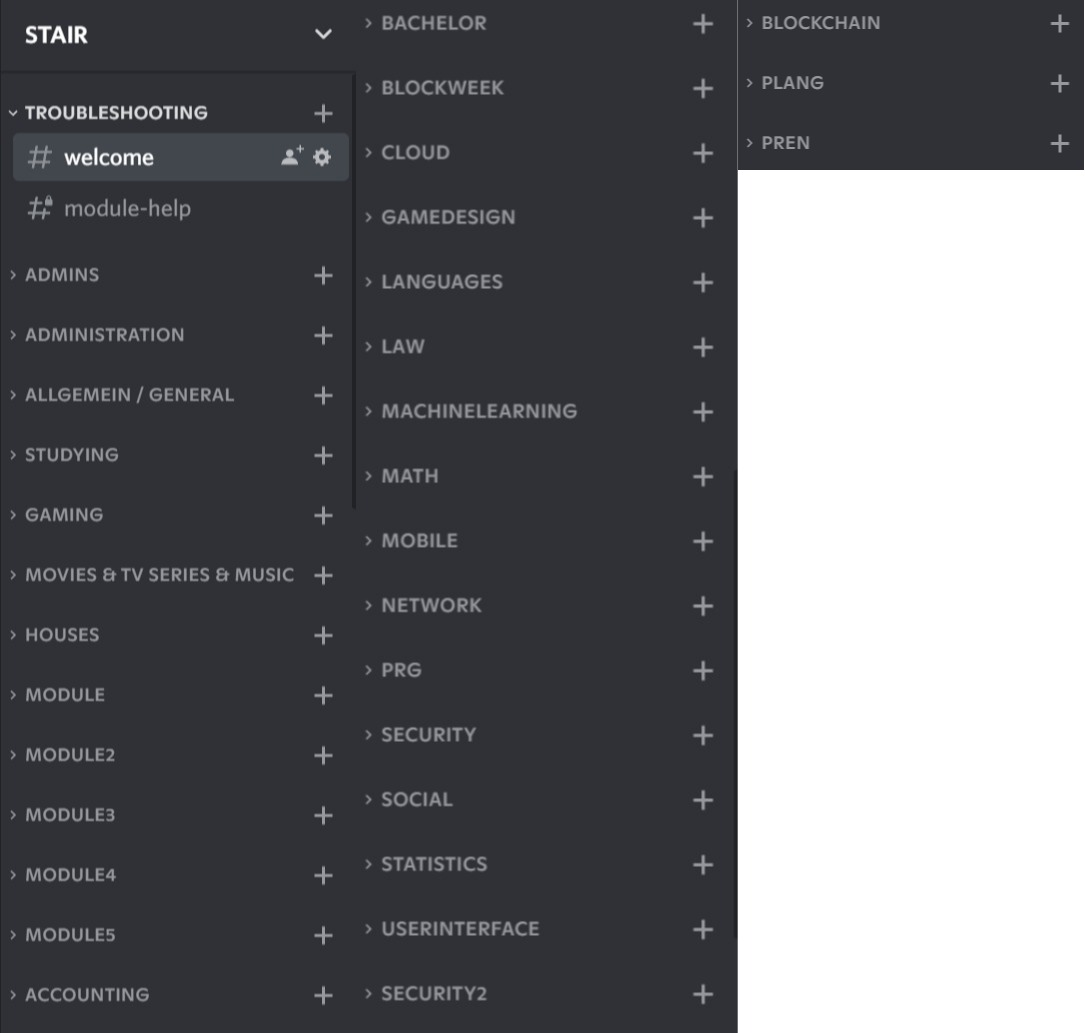
\includegraphics[width=1.0\textwidth,height=10cm]{img/Stair_Discord_Channels.jpg}
    \caption{Stair Discord Channels Alt}
    \label{fig:stair_old_discord_channels}
\end{figure}

\subsubsection*{Ablauf Authentifizierung \& Modulanmeldung}
In den folgenden zwei Seiten wird der Authentifizierungsprozess und der Modulanmeldungsprozess als Ablaufdiagramm beschrieben.
Dieser Ablauf wird zum jetzigen Zeitpunkt durchgeführt.

\begin{landscape}
    \begin{figure}[ht]
        \centering
        \hspace*{-4.1cm}
        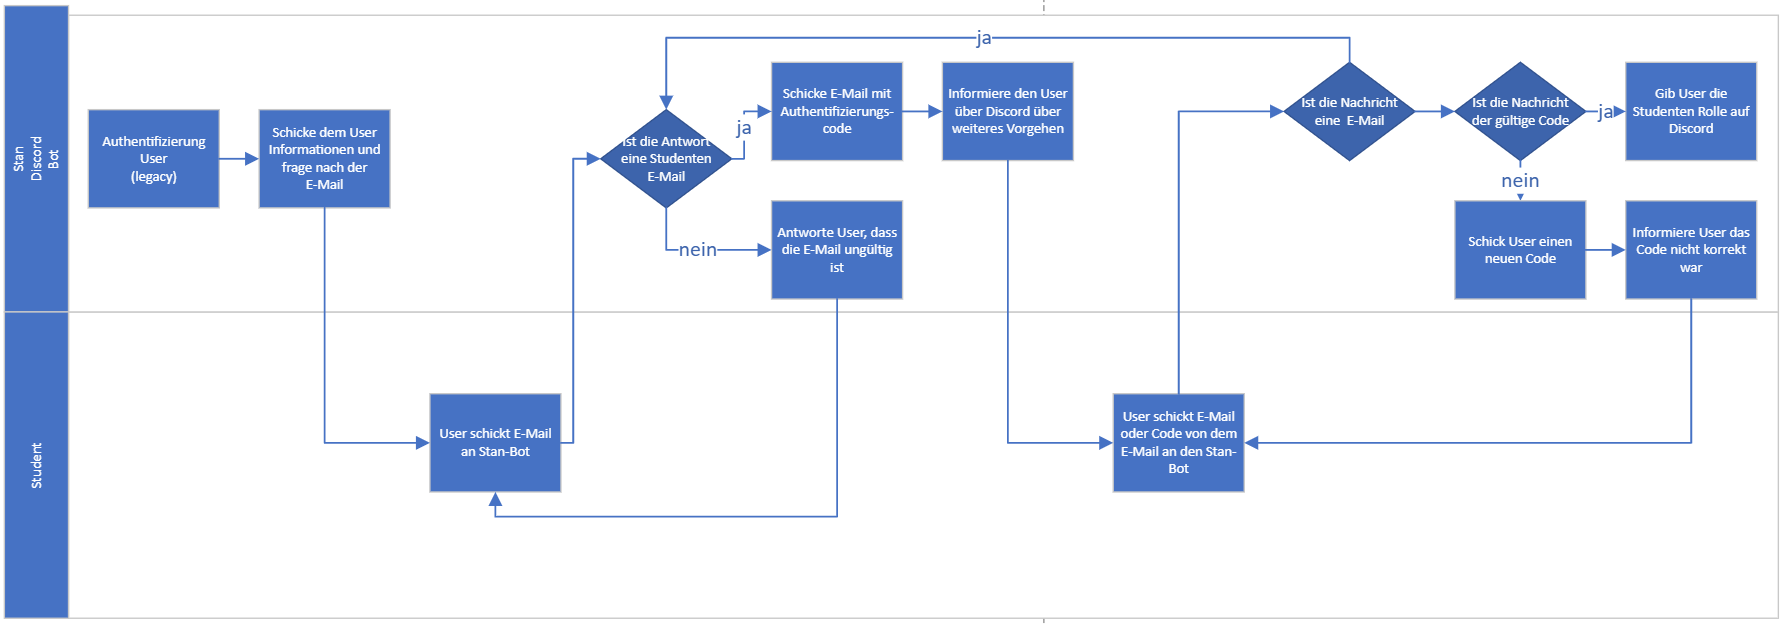
\includegraphics[width=1.9\textwidth]{img/Authentifizierungsprozess_Bot_alt.png}
        \caption{Authentifizierungsprozess Bot alt}
        \label{fig:Authentifizierungsprozess_Bot_alt}
    \end{figure}
    \clearpage
    \begin{figure}[ht]
        \centering
        \hspace*{-4.1cm}
        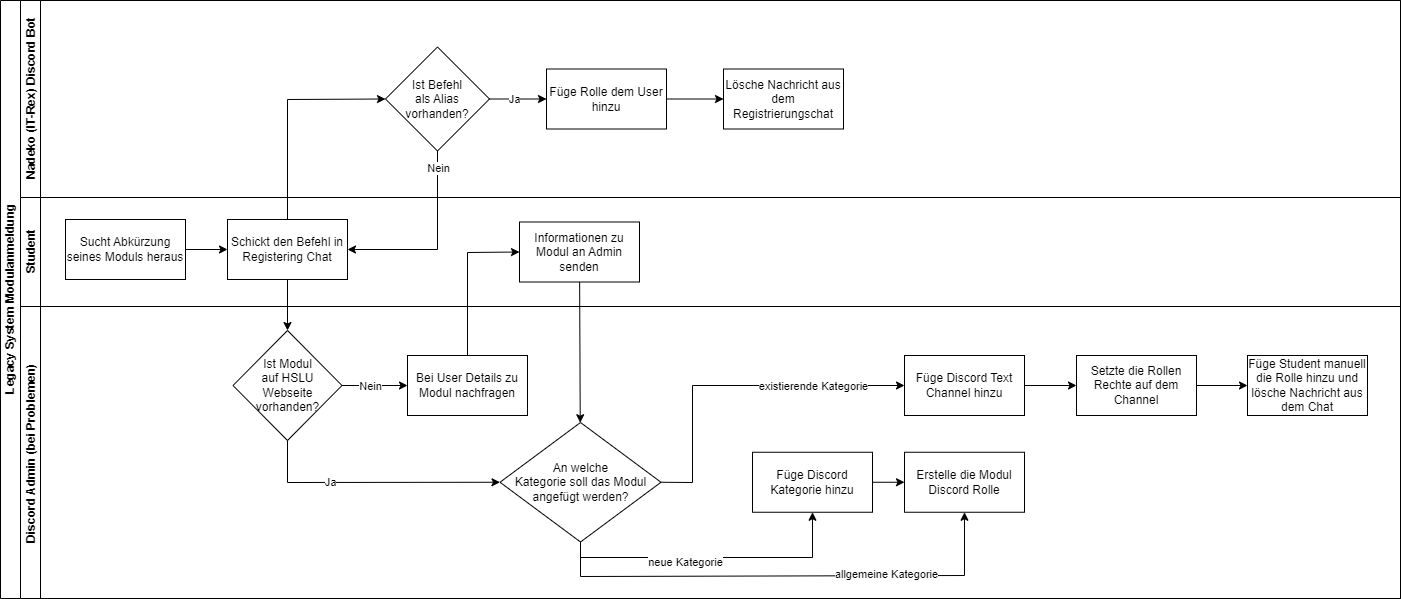
\includegraphics[width=1.9\textwidth]{img/Modulanmeldungsprozess_Bot_alt.png}
        \caption{Modulanmeldungsprozess Bot alt}
        \label{fig:Modulanmeldungsprozess_Bot_alt}
    \end{figure}
\end{landscape}

\subsubsection{Funktionsweise Bot}
Der Bot ist mit der Programmiersprache C\# und dem .NET Framework geschrieben.

\subsubsection*{Konfigurationsmanagement alter Bot}
In der folgenden Tabelle ist eine \"Ubersicht der benutzen IDE, ihrer Spezifizierung und den eingesetzten Libraries.

\begin{table}[h]
    \centering
    \begin{tabular}{|l|p{20em}|l|}
        \hline
        \rowcolor[gray]{.9} Name & Beschreibung & Version \\
        \hline
        .NETCore & Core Library für C\# Projekte.
        Enthält alle grundlegend Klassen und Libraries, welche für die Erstellung von .NET Projekten nötig sind. & 2.0.0 \\
        \hline
        NETStandard Library & Set von Standard .NET APIs & 2.0.3 \\
        \hline
        Discord.NET & Asynchrone API für Discord. & 2.3.0 \\
        \hline
        FakeItEasy & Mocking Bibliothek & 6.0.0 \\
        \hline
        FluentAssertions & Spezifizieren von TDD und BDD-Style Unit Tests. & 5.10.2 \\
        \hline
        Microsoft UserSecrets & User Secret Konfigurations provider & 3.1.0 \\
        \hline
        Microsoft Graph & Erlaubt alle Microsoft Dienste über eine einheitliche Schnittstelle anzusprechen & 1.21.0 \\
        \hline
        Microsoft.Identity.Client & Enthält Binaries für die Microsoft Authentication Library (MSAL) & 4.7.1 \\
        \hline
        Newtonsoft.JSON & High-Performance Framework für JSON & 12.0.3 \\
        \hline
        Ninject & Dependency Injector für .NET Applikationen & 3.3.4 \\
        \hline
        Nito.AsyncEx & Hilfsbibliothek für Task-Based Asynchronous Pattern (TAP) & 5.0.0 \\
        \hline
        Topshelf & Bibliothek zum Hosten von Applikationen. 
        Bietet command-line optionen zum installieren, konfigurieren und laufen lassen von applications as a service. & 4.2.1 \\
        \hline
        xunit & Developer testing framework & 2.4.1 \\
        \hline
    \end{tabular}
    \caption{Konfigurationsmanagement Bot alt}
    \label{tab: Konfigurationsmanagement-Bot-alt}
\end{table}


Das Programm, welches den Bot zur Verfügung stellt, ist nicht gross. Es beinhaltet im Groben einen Client Socket der
Events on Discord abfängt und einer E-Mail Klasse, die E-Mails an den Benutzer versenden kann.
Das Programm ist in zwei Packages aufgeteilt.

\begin{itemize}
    \item StanBot.Core
    \item StanBot.Service
\end{itemize}
\clearpage
\begin{figure}[ht]
    \centering
    \hspace*{-1.5cm}
    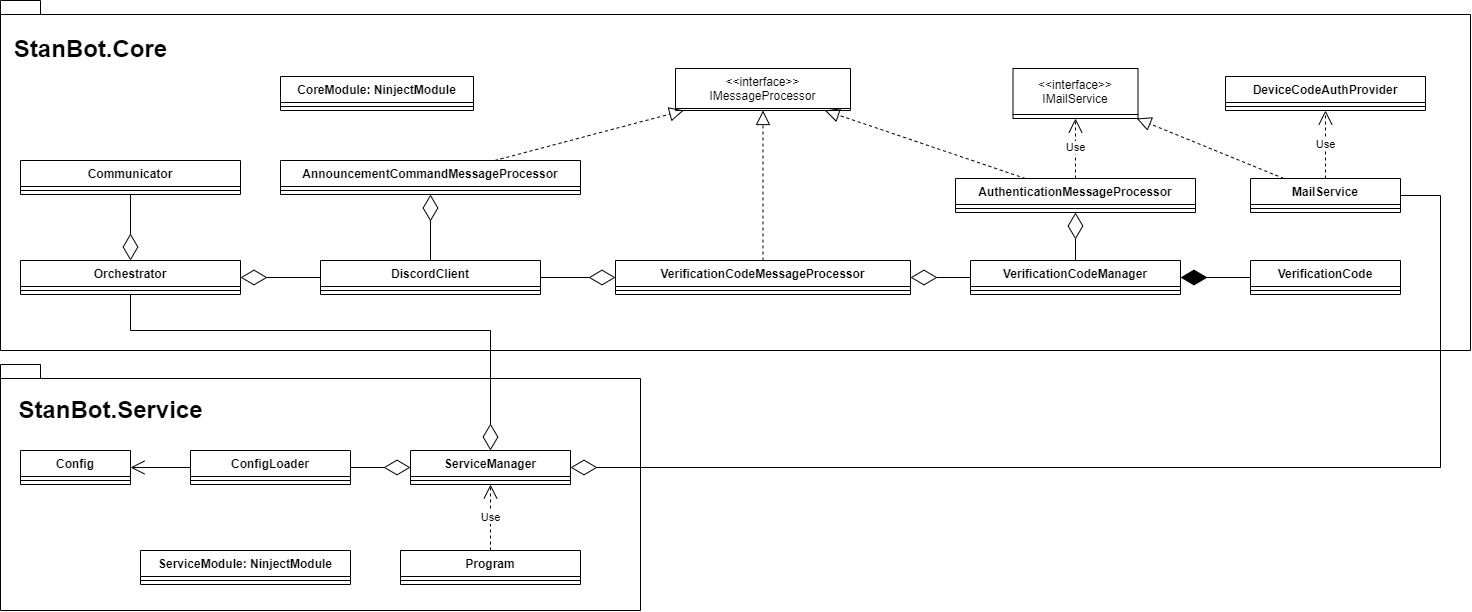
\includegraphics[width=1.2\textwidth]{img/Klassendiagramm_Bot_alt.png}
    \caption{Klassendiagramm Bot alt}
    \label{fig:Klassendiagramm_Bot_alt}
\end{figure}

\subsubsection{Ausführung Bot}
Der Bot läuft auf einem Microsoft Windows Server 2019 Standard auf der Enterprise Lab Umgebung der HSLU. 
Die Konfiguration entspricht der eines Windows Services und läuft dementsprechend durchgehend.

\begin{figure}[hb]
    \centering
    \hspace*{-2.5cm}
    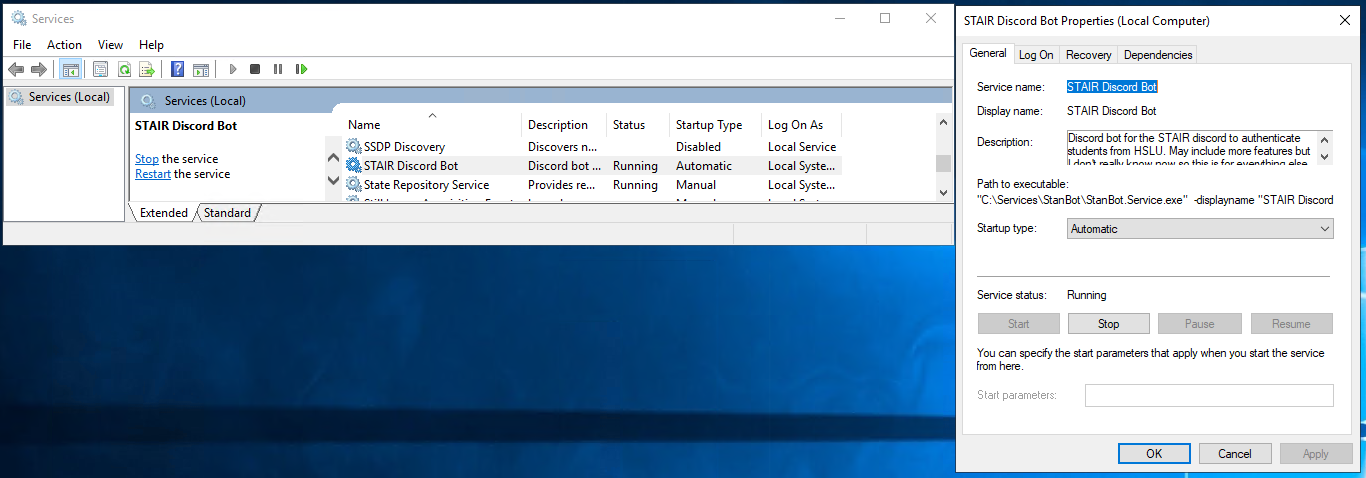
\includegraphics[width=1.3\textwidth,height=6cm]{img/Discord_Bot_old_service_configuration.png}
    \caption{Stair Discord Service Konfiguration Alt}
    \label{fig:bot-service-configuration-old}
\end{figure}
\clearpage

\subsubsection{Geplante Änderungen}\label{geplanteAenderungen}

\subsubsection*{Wechsel zu Linux Server}

Es wurde zusammen mit dem STAIR Team entschieden,
auf Linux zu wechseln um alle Server einheitlich auf Linux zu haben.
Bei STAIR wird noch eine Wordpress-Seite und eine JavaScript Webseite betrieben.
Wordpress ist ein Content Management System (CMS) und wird bei STAIR eingesetzt für die Hauptwebseite mit allen Events und weiteren Informationen.
Da die Projekte jedoch sich von einander stark unterscheiden wurde entschieden mit verschiedenen Servern zu arbeiten und nicht alle auf dem gleichen Server zu hosten.
Gleichzeitig befindet sich die Wordpress-Seite noch auf einem anderen Rechencenter als dem Enterprise Lab der HSLU.
Dies verursacht auch Kosten, welche eingespart werden sollen in der Zukunft.
Um den Transfer zu vereinfachen, macht es sinn, nicht einen ohnehin bald obsoleten Server für das Deployment zu nutzen.

\subsubsection*{Entscheid den Bot neu zu schreiben}

Bei der Analyse des bisherigen Bot wurde bemerkt, dass die veraltete Technologie .NET Standard 2.0 und .NET Core 3.1 mit veralteten Libraries genützt wurden.
Diese werden nicht mehr unterstützt und sollten ersetzt werden.
Für die neue Version wird .NET 6 mit C\# verwendet.
Dies ermöglicht es, inspiration bei der alten Lösung zu holen, falls zum Beispiel die Verwendung der Discord Library unklar ist oder bei einem bereits existierenden Feature ein Probleme auftaucht.
Die neueren .NET Versionen sind Cross-Platform fähig und können damit nun auch auf Linux verwendet werden.\autocite{de_george_installieren_nodate}
Die Sprache wird nicht an der Hochschule breit verwendet, es gibt jedoch ein Modul zu C\#\autocite{} \todo{PDF source is not in Zotero export} und die Sprache ist ähnlich zu Java,
welche grundsätzlich an der Hochschule verwendet wird.
das WIPRO Team war zusätzlich bereits vertraut mit der C\# Sprache und hat diese als angenehm empfunden, was die Entscheidung zusätzlich unterstützte.

\subsubsection*{Entscheid Login Funktionsweise}
\todo{source}
Beim Login wurde überlegt das Switch-Login der Hochschule zu verwenden, welches auch für aussenstehende Zwecke verwendet werden kann.
Hierbei wurde dagegen entschieden, da STAIR nicht die volle Kontrolle über den Service hat und deshalb plötzlich neue Interface Standards erlassen werden können, was zu Problemen führen kann.
Auch muss hierzu ein bestimmter Link geöffnet werden, welcher von Stan verschickt werden muss um die Switch Login Seite zu öffnen.
Dies könnte nicht vertrauenswürdig wirken bei Studenten.
Ausserdem hat sich das Login mittels E-Mails bereits bewährt, weshalb dieses nun weiterhin verwendet wird.

%\subsubsection*{Wechsel zu Community Server}
% https://support.discord.com/hc/en-us/articles/360047132851-Enabling-Your-Community-Server

\subsubsection*{Entscheid zur Anbindung an eine Datenbank}

Eine Datenbank bringt einige Vorteile.
Speziell relevant sind folgende Punkte für dieses Projekt:
\begin{itemize}
    \item Eine Datenbank ermöglicht eine automatische Zuweisung von Studenten zu ihren Häusern.
    \item Sie ermöglicht das automatische markieren von Exstudierenden.
    \item Sie bietet die grösste Erweiterbarkeit für die Zukunft.
    \item Modul-Channels welche zur Zeit nicht gebruacht werden, könnten theoretisch auf Discord gelöscht werden und neu erstellt werden, wenn diese gebraucht werden.
    \item Bei Problemen kann schnell herausgefunden werden, welche genau Person betroffen ist und kann sich auch über alternative Kommunikationswege, wie E-Mail, mit der Person in Kontakt setzen.
    \item Studenten können über ihre E-Mail permanent gebannt werden, ohne dass sie sich mit neuen Discord Accounts wieder anmelden können.
\end{itemize}

Eine Datei wäre ebenfalls möglich zur Datenspeicherung.
Diese hätte jedoch weniger Performance und würde keine Checks durchführen beim Speichern der Daten.
Das Auslesen von gefilterten Daten gestaltet sich ebenfalls einfacher.\autocite{castro_why_2020}
Da bei diesem Projekt wichtig ist, dass die Daten korrekt im Schmea gespeichert werden und die Anpassbarkeit der Datenbank keinen Fokus bekommen hat, wurde eine SQL basierte Datenbank bevorzugt gegenüber von NoSQL Datenbanken.
Als gewählte Technologie hat sich MySQL durch seine grosse Verbreitung sehr gut angeboten.
Online wird MySQL als die zweitmeist genutzte Datenbank-Technologie\\beschrieben.\autocite{noauthor_db-engines_2022}

\subsubsection*{Entscheidung einen eigenen Bot zu entwickeln}
Zusammen mit STAIR wurde entschieden, wieder eine eigensentwickelte Lösung zu wählen.
Dies hat verschiedene Vorteile.
Als erstes ist damit gleich auch der Datenschutz gewährleistet.
Auch sind so keine künstliche Limitierungen eines externen entwickelten Bots vorhanden.
Die einzigen Limitierungen sind vom API von Discord und von technischen Know-How der betreuenden Entwicklern.
Da die verschiedenen Bots eventuell nicht in Europa gehostet sind, könnten Verbindungs- und/oder Performanceprobleme auftreten.
Durch die Log Datei(en) können Fehler einfacher gefunden und nachvollzogen werden.
\newpage
\subsection{Initialisierungsphase}
Aus dem Projektauftrag und aus den Wünschen der Stakeholder werden Anforderungen an das Produkt definiert.
Diese werden für die Realisierungsphase in Epics umgewandelt.
Die Epics werden im Anschluss in einzelne User Stories aufgeteilt, die dann in den Sprints seperat behandelt und gelöst werden.

\subsubsection{Epics}\label{Epics}
Für das Projekt werden folgende Epics definiert.

\begin{table}[h]
    \centering
    \begin{tabular}{ | p{1em} | p{35em} | p{2em} |}
        \hline
        \rowcolor[gray]{.9} ID & Beschreibung & Prio \\
        \hline
        1 & Der Nutzer wird beim erstmaligen Betreten des Discord-Servers vom Bot benachrichtigt.
        Dieser gibt ihm Grundlegende Informationen zum Server und dem Authentisierungsprozess.
        Zu diesem Zeitpunkt hat der Student noch keine Berechtigungen auf dem Server und
        hat nur Zugriff auf den Channel "Help". & A \\
        \hline
        2 & Der Bot soll den Nutzer authentifizieren und mit der Studenten-Rolle versehen können.
        Er kann dabei zwischen den E-Mails von Nicht-Student und Student unterscheiden und auf unvorhergesehene
        Interaktionen, von Seiten des Benutzers, reagieren können. & A \\
        \hline
        3 & Ein Student kann sich beim Bot für ein Modul anmelden. Dieser schaltet den Channel für den Studenten frei,
        so das er darin mit anderen Studierenden kommunizieren kann. Falls das Modul für den Studenten nicht mehr relevant ist,
        kann er es beim Bot wieder abmelden. & A \\
        \hline
        4 & Die Administration des Discord Servers soll einfach neue Modullisten in das System laden können.
        Die neuen oder nicht mehr Verfügbaren Module werden erkannt und entsprechend hinzugefügt oder gelöscht.
        An dem Verhalten des Benutzers soll sich nichts ändern. & A \\
        \hline
        5 & Die Adminsitration kann jedes Semster die neuen Studierenden hinzufügen.
        Diese werden beim potentiellen Authentifizieren direkt in Ihre zugeteilten Häuser-Channels zugewiesen. & A \\
        \hline
        6 & Die Administration von STAIR kann über eine zur Verfügung gestellte Schnittstelle, Statistiken über
        den Discord erstellen. & B \\
        \hline
        7 & Fehlereingaben in dem Modulregistrierungschannel oder interne Fehler vom Bot, sollen direkt automatisch
        an einen hinterlegten Mitarbeiter von STAIR gemeldet werden & C \\
        \hline
    \end{tabular}
    \caption{Epics}
    \label{tab: Epics}
\end{table}

\subsubsection{User Stories}
Die Epics werden in kleinere User-Stories heruntergebrochen und dienen als Bausteine eines Sprints.
Dieser Prozess wird auch \textbf{Story-Splitting} genannt
User-Stories sind immer nach dem gleichen Muster aufgebaut. \\
"Als <Rolle> möchte ich <Ziel/Wunsch>, um <Nutzen>." \\
Die Story muss nicht immer aus der Benutzersicht definiert sein, sondern es können auch technische oder
infrastrukturelle User-Stories so gebildet werden.

In der Strintplannung werden zu jeder User-Story zugehörige Akzeptanzkriterien definiert.
Diese dienen zur Kontrolle, ob die User-Story korrekt umgesetzt wurde und
können auch als Test während der Entwicklung gebraucht werden.
Später können dann die Mitglieder des Teams, den Aufwand der Story realistisch abschätzen.

Gute User-Stories können nach dem Modell \textbf{I.N.V.E.S.T} gebildet werden. \autocite{hammerschall_software_2013} % PMB Projektplanung p.101-103
\begin{itemize}
    \item \textbf{I}ndependent  unabhängig voneinander
    \item \textbf{N}egotiable   zerlegbar, änderbar, kombinierbar, verhandelbar
    \item \textbf{V}aluable     hat wirtschaftlichen Wert
    \item \textbf{E}stimatable  so klar, dass es vom Team geschätzt werden kann
    \item \textbf{S}mall        klein genug, um in einem Sprint entwicklet werden zu können
    \item \textbf{T}estable     klare Akzeptanzkriterien
\end{itemize}

Beim Story-Splitting werden folgende User-Stories für das Projekt definiert.

\begin{longtable}{ | p{1em} | p{16em} | p{13em} | p{2em} | p{3em} | p{2em} |}
    \hline
    \rowcolor[gray]{.9} ID & Beschreibung & Akzeptanzkriterien & Prio & Weight & Sprint \\
    \hline
    1 & Als Bot möchte ich den Benutzer beim ersten Betreten des Server authentifizieren können,
    um ihm die ihm zugeteilten Rollen zuweisen zu können. &
    \tabitem Der Nutzer bekommt beim ersten Betreten des Servers eine Nachricht vom Bot mit Informationen. & A & 12 & 2 \\*
    & & \tabitem Der Student bekommt nach der Anmeldung die Rolle Student zugeteilt und wird dem richtigen Haus-Channel zugewiesen. & & & \\
    \hline
    2 & Als Bot möchte ich den Studenten mittels E-Mail Verifikation authentifizieren können,
    um sicher zu gehen, dass dieser eine gültige Studenten-Mail besitzt. &
    \tabitem Der Student bekommt eine E-Mail auf der Adresse, die er dem Bot mitteilt. & A & 15 & 3 \\*
     & & \tabitem Ein Student kann sich authentifizieren, ein Nicht-Student wird abgewiesen. & & & \\*
     & & \tabitem In der E-Mail steht ein zufällig generierter 6-stelliger Code. & & & \\*
     & & \tabitem Der Bot kann den Code verifizieren, nachdem der Student die E-Mail erhalten hat. & & & \\
    \hline
    3 & Als STAIR Administrator möchte ich neue Studenten einfach erfassen können,
    um sie dem System bekannt zu machen und die Administration zu vereinfachen. &
    \tabitem Neue Studenten können mit ihren zugeteilten Häusern als Liste eingelesen werden & B & 9 & 1 \\*
     & & \tabitem Die neu erfassten Studenten werden im System eingetragen und können für die Authentifizierung verwendet werden. & & & \\
    \hline
    4 & Als Student möchte ich mich für neue Modul-Channels an und abmelden können,
    um mich mit anderen Studenten austauschen zu können. &
    \tabitem Es stehen Befehle im \textbf{Registrierungs-Channel} zur Verfügung, um sich bei Modulen an- und abzumelden. & A & 12 & 3 \\*
     & & \tabitem Der Bot weist den Studenten, bei einer Anmeldung, dem Modul als Mitglied hinzu. & & & \\*
     & & \tabitem Der Bot löscht den Studenten, bei einer Abmeldung, aus der Mitgliederliste,
     so dass der Channel für den Studenten nicht mehr sichtbar ist. & & & \\
    \hline
    5 & Als STAIR Administrator möchte ich Modullisten mit den verfügbaren Modulen, einfach in das System eintragen zu können,
    um sie für den Bot nutzbar zu machen. &
    \tabitem Pro Semester können Modullisten automatisch eingelesen werden. & B & 8 & 2 \\*
     & & \tabitem Neue Module werden automatisch hinzugefügt, und solche, welche nicht mehr Unterrichtet werden, werden gelöscht. & & & \\*
     & & \tabitem Die Module stehen nach dem einlesen direkt bereit, zur Channel-Erstellung durch den Bot. & & & \\
    \hline
    6 & Als STAIR Administrator möchte ich Statistiken aus dem System auslesen können,
    um sie für Marketing oder andere Zwecke gebrauchen zu können. &
    \tabitem Es stehen ein paar vorgefertigte Auslesemöglichkeiten bereit, um sie für den Administrator nutzbar zu machen & C & 9 & 4 \\
    \hline
    7 & Als STAIR Administrator möchte ich sofort benachrichtigt werden, falls mit dem System ewtwas nicht stimmt,
    um Gegenmassnahmen ergreifen zu können. &
    \tabitem Der Administrator wird benachrichtigt, wenn der Bot zu Discord oder zur Datenbank keine Verbindung mehr hat & C & 5 & 5 \\*
     & & \tabitem Der Administrator wird benachrichtigt wenn der E-Mail Versand zur Authentifikation nicht mehr funktioniert. & & & \\
    \hline
    \caption{User-Stories}
    \label{tab: UserStories}
\end{longtable}

\subsubsection*{Sprintplanung}
\begin{table}[h]
    \centering
    \begin{tabular}{|l|l|l|l|}
        \hline
        \rowcolor[gray]{.9} Sprint & Start & Ende & Artefakte \\
        \hline
        Sprint 1 & 10.10.2022 & 16.10.2022 & \tabitem Studentenerfassung implementiert \\
         & & & \tabitem Sprintreview S01 \\
         & & & \tabitem Sprintplannung S02 \\
        \hline
        Sprint 2 & 17.10.2022 & 30.10.2022 & \tabitem Modulerfassung implementiert \\
         & & & \tabitem Sprintreview S02 \\
         & & & \tabitem Sprintplannung S03 \\
        \hline
        Sprint 3 & 31.10.2022 & 13.11.2022 & \tabitem Authentifizierung implementiert \\
         & & & \tabitem Sprintreview S03 \\
         & & & \tabitem Sprintplannung S04 \\
        \hline
        Sprint 4 & 14.11.2022 & 27.11.2022 & \tabitem Statistiken implementiert \\
         & & & \tabitem Sprintreview S04 \\
         & & & \tabitem Sprintplannung S05 \\
        \hline
        Sprint 5 & 28.11.2022 & 11.12.2022 & \tabitem Fehlererkennung implementiert \\
         & & & \tabitem Sprintreview S05 \\
        \hline
    \end{tabular}
    \caption{Sprintplanung}
    \label{tab: Sprintplanung}
\end{table}

Die Projektkontrolle und der Fortschritt wird mit folgenden Tools überwacht.
\begin{itemize}
    \item Github Story-Board (\href{https://github.com/orgs/stairch/projects/1/views/4}{Link zum Story-Board})
    \item Sprintreviews (\nameref{Sprintreviews})
\end{itemize}

\subsubsection{Testdrehbuch}\label{Testdrehbuch}
Wie im Kapitel \nameref{Teststrategie} erwähnt, werden im Folgenden die einzelnen Systemtests beschrieben.
Diese müssen alle manuell vor der Übergabe der Software durchgeführt werden.
\newline
Sie beziehen sich immer auf eine Anforderung / Epic und können so auch bei den einzelnen Sprintreviews zur Kontrolle verwendet werden.
Die Referenzierten Epics sind im Kapitel \nameref{Epics} beschrieben.

\begin{longtable}[ht]{|p{15em}|p{25em}|}
    \hline
    \multicolumn{2}{|l|}{\textbf{Betritt ein neuer Student den Discord-Server, bekommt er direkt eine Nachricht.}} \\*
    \multicolumn{2}{|l|}{\textbf{vom Stan Bot.}} \\
    \hline
    \multicolumn{2}{|l|}{\textbf{Testfall \#1}} \\
    \hline
    \textbf{Epic / Anforderung} & \#1 \\
     & Der Nutzer wird beim erstmaligen Betreten des Discord-Servers vom Bot benachrichtigt.
     Dieser gibt ihm Grundlegende Informationen zum Server und dem Authentifizierungsprozess.
     Zu diesem Zeitpunkt hat der Student noch keine Berechtigungen auf dem Server und
     hat nur Zugriff auf den Channel "Help". \\
    \hline
    \textbf{Durchführung} &
    \begin{enumerate}
        \item Bereitstellen eines Discord Accounts, welcher noch nicht auf dem STAIR-Discord Server angemeldet ist.
        \item Dem STAIR Discord Server beitreten. \url{https://discord.com/invite/Tp7XgzZ}
    \end{enumerate}\\
    \hline
    \textbf{Erwartetes Ergebnis / Verhalten} & Sobald man dem Server beigetreten ist, bekommt man vom Stan Bot eine private Nachricht.
    Dort stehen allgemeine Informationen zum Server und zum Anmeldeprozess. \\
    \hline
    \caption{Testdrehbuch - Testfall \#1}
\end{longtable}

\begin{longtable}[h]{|p{15em}|p{25em}|}
    \hline
    \multicolumn{2}{|l|}{\textbf{Ein Student kann sich beim Bot authentifizieren.}} \\
    \hline
    \multicolumn{2}{|l|}{\textbf{Testfall \#2}} \\
    \hline
    \textbf{Epic / Anforderung} & \#2 \\*
     & Der Bot soll den Nutzer authentifizieren und mit der Studenten-Rolle versehen können. \\
    \hline
    \textbf{Durchführung} &
    \begin{enumerate}
        \item Der Student hat eine Nachricht von Stan als Direkt Nachricht erhalten.
        \item Der Student schickt dem Bot seine E-Mail Adresse nach dem Muster \textit{<name.vorname>@stud.hslu.ch} .
        \item Nach Erhalt der E-Mail, schickt der Student, Stan den 6-stelligen Verifizierungscode.
    \end{enumerate}\\
    \hline
    \textbf{Erwartetes Ergebnis / Verhalten} & Der Student sollte nach Senden seiner E-Mail Adresse dem Bot, eine E-Mail von ihm erhalten.
    In dieser ist ein zufällig generierter 6-stelliger Verifizierungscode enthalten.
    Nach dem verifizieren, bekommt der Nutzer die Rolle Student und "Haus" zugeteilt und hat Zugriff auf die Grund-Channels. \\
    \hline
    \caption{Testdrehbuch - Testfall \#2}
\end{longtable}

\begin{longtable}[h]{|p{15em}|p{25em}|}
    \hline
    \multicolumn{2}{|l|}{\textbf{Ein Nicht-Student kann sich nicht authentifizieren.}} \\
    \hline
    \multicolumn{2}{|l|}{\textbf{Testfall \#3}} \\
    \hline
    \textbf{Epic / Anforderung} & \#2 \\*
     & Er kann dabei zwischen den E-Mails von Nicht-Student und Student unterscheiden und
     auf unvorhergesehene Interaktionen, von Seiten des Benutzers, reagieren können. \\
    \hline
    \textbf{Durchführung} &
    \begin{enumerate}
        \item Ein Nicht-Student schickt dem Bot eine E-Mail, welche sich vom Muster \textit{<name.vorname>@stud.hslu.ch} unterscheidet.
    \end{enumerate}\\
    \hline
    \textbf{Erwartetes Ergebnis / Verhalten} & Der Nutzer bekommt direkt eine Nachricht vom Bot, das diese E-Mail nicht gültig ist.
    Es können sich nur Studenten authentifizieren. \\
    \hline
    \caption{Testdrehbuch - Testfall \#3}
\end{longtable}

\begin{longtable}[h]{|p{15em}|p{25em}|}
    \hline
    \multicolumn{2}{|l|}{\textbf{Ein STAIR Administartor kann eine Liste mit Studenten in das System einlesen.}} \\
    \hline
    \multicolumn{2}{|l|}{\textbf{Testfall \#4}} \\
    \hline
    \textbf{Epic / Anforderung} & \#5 \\*
     & Die Adminsitration kann jedes Semester die neuen Studierenden hinzufügen.
     Diese werden beim potentiellen Authentifizieren direkt in Ihre zugeteilten Häuser-Channels zugewiesen. \\
    \hline
    \textbf{Durchführung} &
    \begin{enumerate}
        \item Der STAIR Administrator muss sich eine Liste von Studenten mit zugehörigen Häusern von der Hochschul-Administration besorgen.
        \item Er kann die Liste als Parameter an ein "LoadStudent" Script übergeben.
    \end{enumerate}\\
    \hline
    \textbf{Erwartetes Ergebnis / Verhalten} & Die Liste wird automatisch in das System eingelesen und die entsprechenden Datenbankeinträge werden erstellt.
    Studenten, welche das letzte Semester bestanden haben und nicht mehr auf der Liste vorhanden sind, werden als Ex-Studenten markiert.\\
    \hline
    \caption{Testdrehbuch - Testfall \#4}
\end{longtable}

\begin{longtable}[h]{|p{15em}|p{25em}|}
    \hline
    \multicolumn{2}{|l|}{\textbf{Ein STAIR Administrator kann eine Liste mit Modulen in das System einlesen.}} \\
    \hline
    \multicolumn{2}{|l|}{\textbf{Testfall \#5}} \\
    \hline
    \textbf{Epic / Anforderung} & \#4 \\*
     & Die Administration des Discord Servers soll einfach neue Modullisten in das System laden können.
     Die neuen oder nicht mehr verfügbaren Module werden erkannt und entsprechend hinzugefügt oder gelöscht.
     An dem Verhalten des Benutzers soll sich nichts ändern. \\
    \hline
    \textbf{Durchführung} &
    \begin{enumerate}
        \item Der STAIR Administrator muss sich eine Liste mit allen verfügbaren Modulen des Departements Informatik von der Hochschul-Administration besorgen.
        \item Er kann die Liste als Parameter an ein "LoadModules" Script übergeben.
    \end{enumerate}\\
    \hline
    \textbf{Erwartetes Ergebnis / Verhalten} & Alle Module sollen in das System eingelesen werden und
    die entsprechenden Datenbankeinträge werden erstellt.
    Neue Module werden automatisch hinzugefügt.
    Module, welche nicht mehr auf der Liste vorhanden sind, werden gelöscht. \\
    \hline
    \caption{Testdrehbuch - Testfall \#5}
\end{longtable}

\begin{longtable}[h]{|p{15em}|p{25em}|}
    \hline
    \multicolumn{2}{|l|}{\textbf{Ein Student kann sich beim Bot für ein Modul anmelden.}} \\
    \hline
    \multicolumn{2}{|l|}{\textbf{Testfall \#6}} \\
    \hline
    \textbf{Epic / Anforderung} & \#3 \\*
     & Ein Student kann sich beim Bot für ein Modul anmelden.
     Dieser schaltet den Channel für den Studenten frei, so, dass er darin mit anderen Studierenden kommunizieren kann. \\
    \hline
    \textbf{Durchführung} &
    \begin{enumerate}
        \item Der Student geht auf den Registrierungs-Channel.
        \item Er schreibt \textit{show <module>} in den Chat. (Also z.B. \textit{show ISF})
    \end{enumerate}\\
    \hline
    \textbf{Erwartetes Ergebnis / Verhalten} & Der Bot erkennt das Modul und fügt den Studenten automatisch als Mitglied diesem Text-Channel hinzu.
    Der Channel ist nun für den Studenten sichtbar. \\
    \hline
    \caption{Testdrehbuch - Testfall \#6}
\end{longtable}

\begin{longtable}[h]{|p{15em}|p{25em}|}
    \hline
    \multicolumn{2}{|l|}{\textbf{Ein Student kann sich beim Bot bei einem Modul abmelden.}} \\
    \hline
    \multicolumn{2}{|l|}{\textbf{Testfall \#7}} \\
    \hline
    \textbf{Epic / Anforderung} & \#3 \\*
     & Falls das Modul für den Studenten nicht mehr relevant ist, kann er es beim Bot wieder abmelden. \\
    \hline
    \textbf{Durchführung} &
    \begin{enumerate}
        \item Der Student geht auf den Registrierungs-Channel.
        \item Er schreibt \textit{hide <module>} in den Chat. (Also z.B. \textit{hide ISF})
    \end{enumerate}\\
    \hline
    \textbf{Erwartetes Ergebnis / Verhalten} & Der Bot erkennt das Modul und meldet den Studenten automatisch davon ab.
    Dies entfernt ihn von der Mitgliederliste des Channels und wird dadurch für ihn wieder nicht einsehbar. \\
    \hline
    \caption{Testdrehbuch - Testfall \#7}
\end{longtable}

\begin{longtable}[h]{|p{15em}|p{25em}|}
    \hline
    \multicolumn{2}{|l|}{\textbf{Ein STAIR Administrator kann über ein Script Statistiken auslesen.}} \\
    \hline
    \multicolumn{2}{|l|}{\textbf{Testfall \#8}} \\
    \hline
    \textbf{Epic / Anforderung} & \#6 \\*
     & Die Administration von x kann über eine zur Verfügung gestellte Schnittstelle, Statistiken über den Discord erstellen. \\
    \hline
    \textbf{Durchführung} &
    \begin{enumerate}
        \item Der STAIR Administrator kann sich mit dem Script "Statistics" über die verschiedenen Statistiken informieren.
        \item Er kann einen Befehl auf diesem Script ausführen.
    \end{enumerate}\\
    \hline
    \textbf{Erwartetes Ergebnis / Verhalten} & Je nach Befehl gibt das Script die gewünschten Werte zurück.
    So können zum Beispiel die Anzahl Studenten pro Haus, oder die momentanen Modulanmeldungen ausgelesen werden. \\
    \hline
    \caption{Testdrehbuch - Testfall \#8}
\end{longtable}
\clearpage

\subsection{Konfigurationsmanagement C\# Solution}
In der folgenden Tabelle werden alle verwendeten NuGet Packete mit der verwendeten Version aufgelistet.

\begin{table}[h]
    \centering
    \begin{tabular}{|l|p{20em}|l|}
        \hline
        \rowcolor[gray]{.9} Name & Beschreibung & Version \\
        \hline
        .NET Core & Core Library für C\# Projekte.
        Enthält alle grundlegend Klassen und Libraries, welche man zum Erstellen von .NET Applikationen benötigt. & 6.0.0 \\
        \hline
        Discord.Net & Asynchronous API für Discord & 3.8.1 \\
        \hline
        linq2db.Mysql & Arbeiten mit Linq und Mysql für .NET & 4.3.0 \\
        \hline
        Micosoft Systemd & .NET hosting Infrastruktur für Systemd Services & 7.0.0 \\
        \hline
        Microsoft Graph & Erlaubt alle Microsoft Dienste über eine einheitliche Schnittstelle anzusprechen & 4.48.0 \\
        \hline
        Microsoft.NET.Test.Sdk & MSbuild targets für .NET Test Projekte. & 17.1.0 \\
        \hline
        MSTest & Evolution von Microsofts Test Framework & 2.2.8 \\
        \hline
        NLog.Extensions.Logging & Logging Framework für .NET Applikationen & 5.2.0 \\
        \hline
        ScottPlot & Plottion Library für .NET Applikationen & 4.1.59 \\
        \hline
        coverlet.collector & Code coverage library & 3.1.2 \\
        \hline
    \end{tabular}
    \caption{Konfigurationsmanagement}
    \label{tab: Konfigurationsmanagement}
\end{table}

Man kann diese NuGet Packete für die ganze Solution installieren, oder für einzelne Projekte.
Im folgenden wird aufgelistet, welches Projekt welche Packete enthält.\\
Ganze Solution:
\begin{itemize}
    \item NLog
\end{itemize}
StanBot Projekt:
\begin{itemize}
    \item Discord.Net
    \item Micosoft Systemd
    \item Microsoft Graph
    \item ScottPlot
\end{itemize}
StanDatabase Projekt:
\begin{itemize}
    \item linq2db.Mysql
\end{itemize}
StanDatabaseTest Projekt
\begin{itemize}
    \item coverlet.collector
    \item Microsoft.NET.Test.Sdk
    \item MSTest
\end{itemize}

\newpage
\subsection{Sprint 1}
Zum Start von Sprint 1 sieht der aktuelle Sprint Plan mit den User-Stories wie folgt aus.
\begin{figure}[h]
    \centering
    \hspace*{-2cm}
    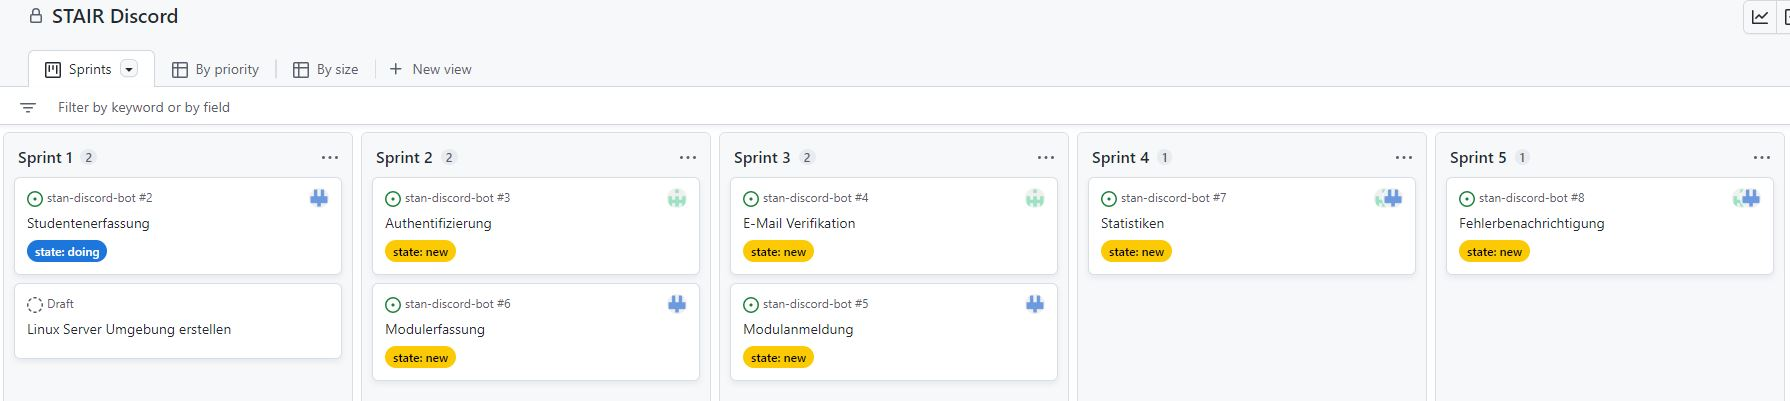
\includegraphics[width=1.3\textwidth]{img/Start_Sprint1_Stories.jpg}
    \caption{Start Sprint 1 User Stories}
    \label{fig:start_sprint_one}
\end{figure}

In der Abbildung erkennt man, dass sich Sprint 1 mit der Studentenerfassung und
mit dem Aufsetzen der Linux Umgebung befasst.

\subsubsection{Entity Relationship Diagramm}\label{entity-relationship-diagramm}
Um die Software Architektur richtig planen zu können, muss im Vorfeld festgelegt werden,
welche Daten im System wichtig sind und wie diese gespeichert werden.
Um diesen Zusammenhang richtig darstellen zu können, wird ein Entity-Relationship Diagramm (ERD) erstellt.
Das ERD kann später in ein Datenbank Schema übertragen werden.
Die einzelnen Tabellen sind wie folgt beschrieben.

\begin{figure}[h]
    \centering
    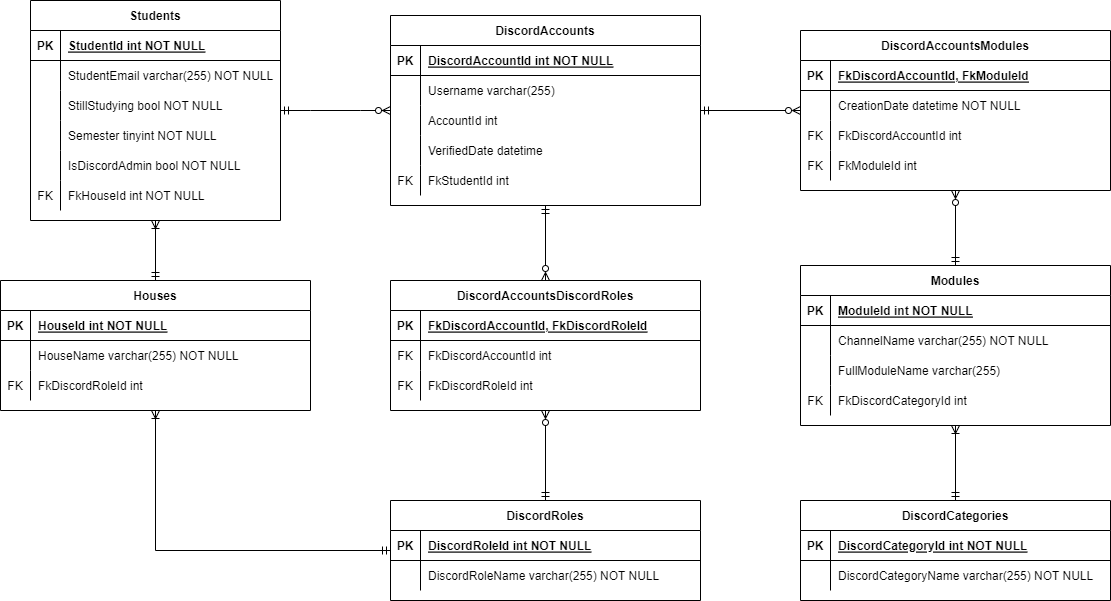
\includegraphics[width=1\textwidth]{img/ER-Diagramm.png}
    \caption{Entity Relationship Diagram}
    \label{fig:ER-Diagram}
\end{figure}

(Ein grosses Bild des Diagramms findet sich im Anhang auf Seite \pageref*{fig:ER-Diagram-big})\\
Bei der Datenspeicherung wird eine Unterteilung zwischen dem Studenten und seinem Discord Account vorgenommen.
Dies erlaubt es, eine saubere Trennung zwischen den richtigen Studenten und ihrem Online erscheinen auf Discord zu gewährleisten.
(Seperation of Concerns (SOC)).
Die Studentendaten, wie Name, Vorname, E-Mail Adresse und Hauszuteilung, werden von der Hochschul-Administration zur Verfügung gestellt und können als Liste eingelesen werden.
Dabei werden die Tabellen \textit{Student} und \textit{House} aufgefüllt und die Zuordnung gemacht.
Implementiert wird die Funktionalität in diesem Sprint 1 (\nameref{tab: UserStories}).
\newline
Der \textit{DiscordAccount} wird bei der Authentifikation dem Studenten zugeordnet.
Über die Tabelle \textit{AccountRole}, werden nach dem Authentifizierungsprozess dem Studenten, die richtigen Rollen zugeordnet.
\newline
Die Tabelle \textit{Module} wird auch über eine, von der Hochschul-Administration, zur Verfügung gestellte Liste befüllt.
Wenn nun der Student sich im Discord beim Bot für ein Modul anmeldet, wird die Zuordnung von Modul und DiscordAccount vorgenommen.
Der richtige Student, bzw. seine Daten, haben mit dieser Zuteilung nichts zu tun.
\newline
Die Tabelle \textit{Category} ist für die technische Umsetzung der Modulgestaltung in Discord möglich.
Durch die Einschränkung von 50 Channeln in einer Kategorie \ref{discord_einschraenkungen}, können nicht alle Module in einer Kategorie zusammengafsst werden.
Dies bedeutet das die Module aufgeteilt werden müssen.
In dieser Tabelle werden die Anzahl Kategorien gespeichert.

\subsection{Aufsetzen Solution}
Die C\# Solution wird in drei Projekte aufgeteilt, welche jeweils andere Verantwortlichkeiten haben.
\begin{itemize}
    \item StanBot
    \item StanDatabase
    \item StanScripts
    \item StanDatabaseTest
\end{itemize}

In dem \textbf{StanBot} Projekt wird der Discord Bot erstellt und alle Funktionalität liegen,
die mit dem Bot zusammenhängt.\\
In dem \textbf{StanDatabase} Projekt wird die Datenbank Anbindung verwaltet.
Darin werden die Tabellen der Datenbank auf zugeweisene Klassen gemappt.
Mithilfe der Library LinQ2DB werden die Tabellen der Datenbank, dann über diese Klassen verwaltet.
Datenbank Operationen sollen nur in diesem Projekt erfolgen. 
Die anderen Projekte sollen keinen direkten Zugriff auf die Datenbank haben.\\
Das \textbf{StanScripts} Projekt wird alle Scripte enthalten, 
die für die Verwaltung des Discord Servers und der Datenbank nötig sind.
Darin werden sich die Scripte für die Studenten -und Modulerfassung befinden.\\
Im \textbf{StanDatabaseTest} Projekt werden die Tests für die Datenbank geschrieben.
In .NET Applikationen ist es üblich ein eigenes Projekt für die Tests zu erstellen.\autocite{tdykstra_organisieren_nodate}

\subsubsection{Repository Pattern für die Daten}
Wie im vorherigen Kapitel erwähnt, soll nur das StanDatabase Projekt direkten Zugriff auf die Datenbank haben.
Wenn der Discord Bot, oder ein Script, Datenbankoperationen ausführen will, wird dazu das Repository Pattern verwendet.\\
Das Repository Pattern ist dazu da, die Create, Read, Update und Delete (CRUD) Funktionen, 
welche auf Tabellen durchgeführt werden, zu kapseln. \autocite{gosebrink_aspnet_2014}
Es sieht vor, dass jedes Objekt genau eine Schnittstelle hat, über die Veränderung daran vorgenommen werden können.

\begin{figure}[h]
    \centering
    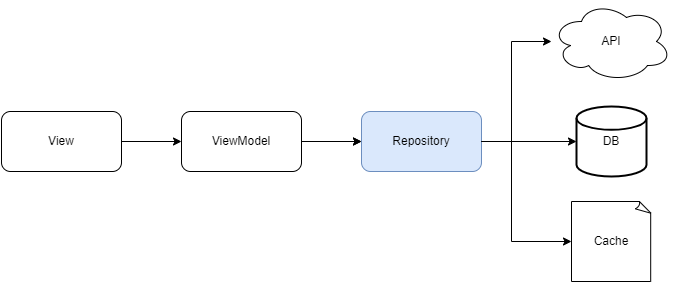
\includegraphics[width=1\textwidth,height=5cm]{img/Repository_Pattern.png}
    \caption{Darstellung Repository Pattern}
    \label{fig:repository_pattern}
\end{figure}
%https://www.google.ch/url?sa=i&url=https%3A%2F%2Fmedium.com%2Fcorebuild-software%2Fandroid-repository-pattern-using-rx-room-bac6c65d7385&psig=AOvVaw3r0fNPN8XItp0pPq7KFvUP&ust=1668526531304000&source=images&cd=vfe&ved=0CBAQjRxqFwoTCMiumpaDrvsCFQAAAAAdAAAAABAD

Wie in der Darstellung zu erkennen, gibt es für andere Klassen nur noch einen Zugriffspunkt für das gewünschte Datenobjekt.
\newline
Ein weiterer Vorteil dieses Patterns ist die vereinfachte Testbarkeit.
Da das Repository selbst eine Schnittstelle, also ein Interface ist, kann es meherere Implementationen davon geben.
Für die richtige Applikation kann nun eine Implementation erstellt werden, die wirklich Daten auf der Datenbank verändert,
und für das Testen kann eine Implementation erstellen werden, die nur Mock Daten enthält.\\
Mithilfe von Dependency Injection kann nun jeweils die gewünschte Implementation für das Repository übergeben werden.

\begin{lstlisting}[language=csharp]
// IHouseRepository
public interface IHouseRepository
{
    House GetHouseByName(string houseName);
    bool IsHouseNameValid(string houseName);
}


// HouseRepositoryImpl
public class HouseRepository : IHouseRepository
{
    public House GetHouseByName(string houseName)
    {
        using (var db = new DbStan()) { ... }
    }

    public bool IsHouseNameValid(string houseName)
    {
        using (var db = new DbStan()) { ... }
    }
}

// LoadStudentScript
public class LoadStudents
{
    private readonly IHouseRepository _houseRepository;
    public LoadStudents(IHouseRepository houseRepository)
    {
        _houseRepository = houseRepository;
    }

    public void LoadStudentsFromFile(string filePath)
    {
        ...
        _houseRepository.GetHouseByName(values[houseIndex]);
        ...
    }
}

// Program
public static class Program
{
    public static void Main(string[] args)
    {
        LoadStudents loadStudents = new LoadStudents(new HouseRepository());
        loadStudents.LoadStudentsFromFile(args[1]);
    }
}
\end{lstlisting}

\subsubsection{Studentenerfassung}

Die Studenten werden über ein vordefiniertes CSV File geladen.
Nach dem Laden der Datei kann entschieden werden, ob die zuvor erfassten Nutzer als Exstudenten markiert werden sollen.
Dies ermöglicht, gleich wie bei den Modulen, Studenten zu ergänzen und zum Start des neuen Semesters die Exstudierenden als solche zu markieren in der Datenbank.
Zum Schluss muss über Discord noch ein Befehl gestartet werden um die Rollen auf dem Discord aktualisieren zu können.
Das CSV Format, sowie der Discord- und Konsolen-Befehl werden im Kapitel \nameref{Bedienungsanleitung} genauer beschrieben.

\subsubsection{Aufsetzen der Linux Umgebung}

Der Ubuntu Server wurde vom Enterprise Lab aufgesetzt.
In der Anleitung im Kapitel \nameref{Bedienungsanleitung} wird die genaue Installation erklärt.
Bei der Installation stellte MySQL das grösste Problem dar, da diese ein Standardpasswort setzt ohne dies dem Nutzer mitzuteilen was ses ist.
Dieses muss deshalb mühsam herausgelesen werden aus dem Log Output.

\subsubsection{Verbinden der Datenbank mit Linq2DB}

Die Verbindung zur Datenbank funktioniert über einen Connection String.
Dieser beinhaltet die Adresse des Datenbank Servers, den dazugehörigen Port, den Datenbank Namen, den Benutzer, das Passwort, sowie das Encoding.
Das genaue Format wird in der Anleitung im Kapitel \nameref{konfigurationStanBot} beschrieben.

\newpage
\subsection{Sprint 2}
In diesem Sprint wird sich mit der Modulerfassung per Script beschäftigt,
dem Erstellen des Discord Bots und der ersten Kommunikation damit.

\subsubsection{Modulerfassung}

Für die Modulerfassung wird die Liste an Modulen vom Sekretariat benötigt.
Diese muss dann auf den Server hochgeladen werden und kann dann mithilfe der StanScripts Anwendung eingelesen werden.
Nach dem Einlesen kann entschieden werden, ob die bereits zuvor erfassten Module gelöscht werden sollen oder nicht.
Dies ermöglicht es dem Administrator einzelne fehlende Module nachzuerfassen oder vor dem Start des neuen Semesters die alten nicht mehr existierenden Module zu entfernen.
Das Format der einzulesenden CSV-Datei wird im Kapitel \nameref{Bedienungsanleitung} geschrieben.

\subsubsection{Aufsetzen Discord Bot}
Um einen Bot zu erstellen, muss man eine Applikation auf der online Discord Developer Plattform kreieren.
Dort kann man den Namen des Bots angeben und erhält ein Application Token.
\begin{figure}[h]
    \centering
    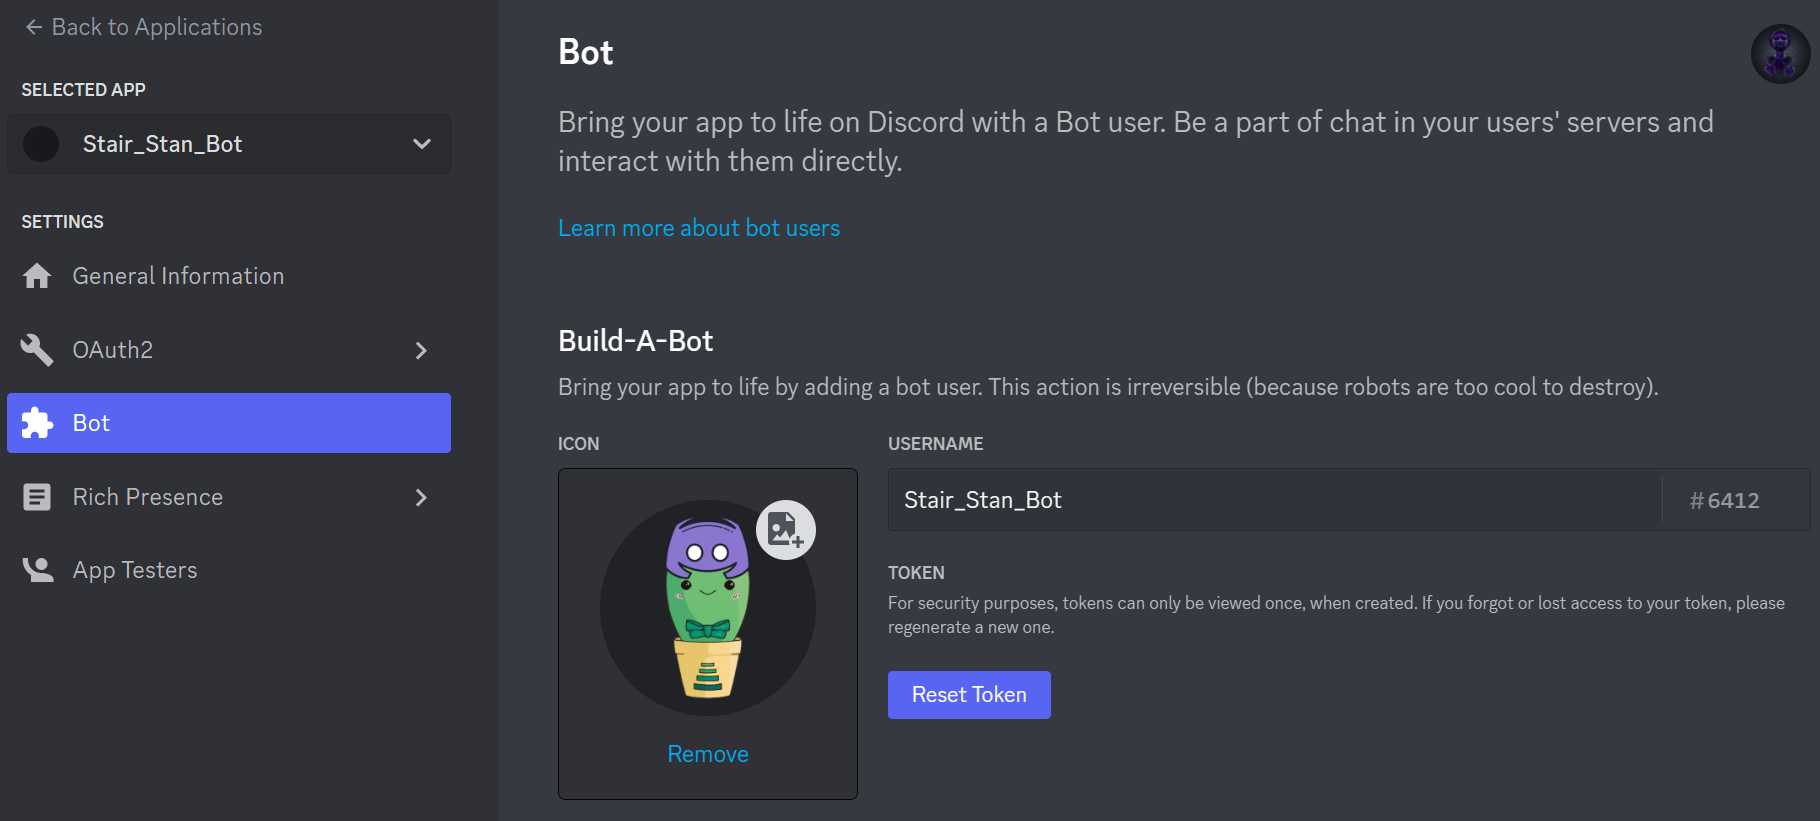
\includegraphics[width=1\textwidth]{img/discord_developer_bot.png}
    \caption{Developer Page Discord Application Token}
    \label{fig:delevoper-application-token}
\end{figure}
Dieses dient wie als Private Key der Applikation und wird verwendet um sich im Code mit dem Bot zu verbinden.
Weiter müssen auf der Platform noch die Berechtigungen des Bots spezialisiert werden.
Dies kann unter dem Tab OAuth2 -> URL Generator gemacht werden.
Die zugewisenen Berechtigungen müssen gut überlegt sein, da man nur für spezifizierte Events, Callbacks im Code bekommt.
Für dieses Projekt muss die Berechtigung Administrator vergeben werden.
Dies sollte allerdings immer mit Vorsicht genossen werden.
Da der Stan Bot private Channels erstellen und verwalten soll, benötigt er diese Berechtigung.
Wenn man die gewünschten Berechtigungen markiert hat, erhält man eine URL.
Diese kann man direkt im Browser eingeben, um den Bot einem Server zuzuordnen.
Damit das gelingt, muss der Nutzer auf dem Server die Berechtigung zum Bots hinzufügen besitzen. 

\begin{figure}[h]
    \begin{minipage}[t]{0.5\textwidth}
        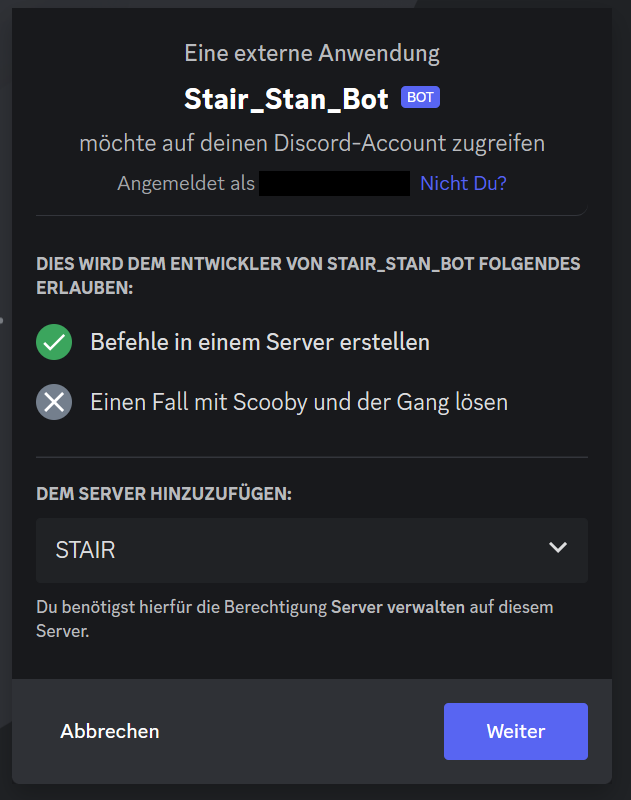
\includegraphics[width=0.7\textwidth]{img/apply_bot_to_server.png}
    \end{minipage}
    \begin{minipage}[t]{0.5\textwidth}
        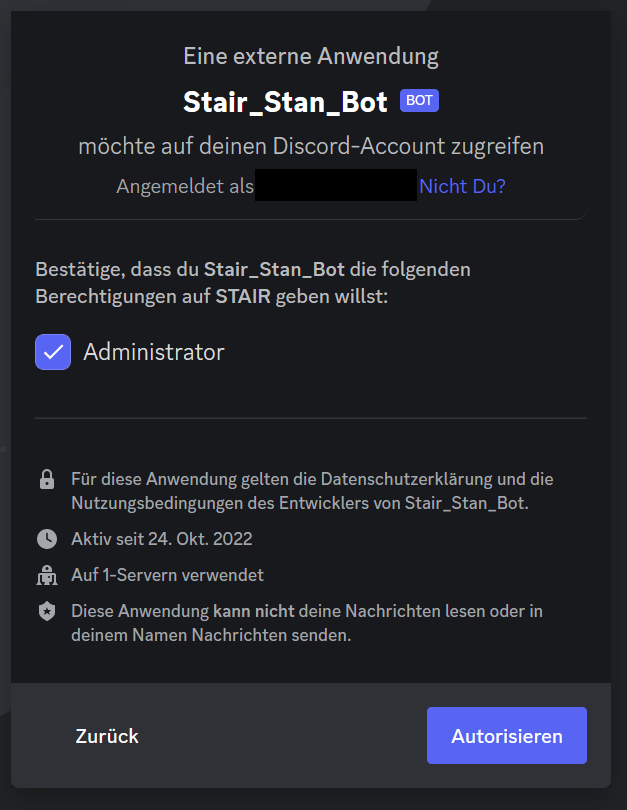
\includegraphics[width=0.7\textwidth]{img/apply_bot_to_server_2.png}
    \end{minipage}
    \caption{Bot dem Server hinzufügen}
    \label{fig:apply-bot-to-server}
\end{figure}

\subsubsection{Stan Bot Architektur}
Grundlegend geht es bei der Bot Architektur um die Kommunikation mit der DiscordClient Klasse.
Diese dient als Client-Komponente des Bots und man kann sich dort auf alle Events abonnieren, die Discord anbietet.\\

\subsubsection*{Services und Dependency Injection}
In der Main-Methode der Applikation wird ein Host Environment für die Applikation erstellt.
Dieses Environment braucht man, damit der Bot später als Deamon auf der Linux Umgebung im Hintergrund laufen kann.
Des weiteren bietet es noch Funktionen zur Dependency Injection an.
Alle Klassen können dort als Singleton, Scoped oder Transient registriert werden.
Aus der Microsoft .NET Dokumentation:
\textit{
\begin{itemize}
    \item Transient-Vorgänge sind immer unterschiedliche, und mit jedem Abruf des Diensts wird eine neue Instanz erstellt.
    \item Scoped-Vorgänge ändern sich nur durch einen neuen Bereich, die Instanz ist jedoch innerhalb eines Bereichs immer gleich.
    \item Singleton-Vorgänge sind immer gleich, und eine neue Instanz wird nur einmal erstellt. \autocite{ievangelist_verwenden_nodate}
\end{itemize}
}

\begin{lstlisting}[language=csharp]
// Program.cs
using IHost host = Host.CreateDefaultBuilder()
            .ConfigureServices((_, services) => services
                .AddSingleton(new DiscordSocketClient())
                .AddSingleton<EventHandler>()
                .AddScoped<IStudentRepository, StudentRepository>()
            .Build();
\end{lstlisting}

In der Bot Klasse kann nun mithilfe eines Providers des Host Environments, die Instanz des gebrauchten Services geholt werden.

\begin{lstlisting}[language=csharp]
// Bot.cs
using IServiceScope serviceScope = _hostEnvironment.Services.CreateScope();
IServiceProvider provider = serviceScope.ServiceProvider;
_discordSocketClient = provider.GetRequiredService<DiscordSocketClient>();
\end{lstlisting}

Die Klasse kann aber auch direkt in einen Konstruktor \textit{Injected} werden.
Auf diese Weise hat man an einer Stelle die Kontrolle über alle verfügbaren Klassen und Instanzen.
\begin{lstlisting}[language=csharp]
// EventHandler.cs
public class EventHandler
{
    private readonly DiscordSocketClient _discordSocketClient;
    public EventHandler(DiscordSocketClient discordSocketClient)
    {
        _discordSocketClient = discordSocketClient;
    }
}
\end{lstlisting}

\subsubsection*{Laden der Config}
Beim Starten des Discord Bots muss eine Konfiguration mit spezifischen \textbf{DiscordApplicationToken} mitgegeben werden.
Dieses Application Token ist wie der Private Key der Applikation und sollte nicht veröffentlicht werden.
Um diese und weitere sensible Informationen einlesen zu können, wird die Config Klasse erstellt.\\
Diese enthält alle Felder der Settingsdatei und dient als Zugriffspunkt für die sensiblen Informationen.
Sie liest mit einem einfachen JSON-Parser die Settings Datei ein und setzt ihre Attribute.
Dabei werden zwei Settingsfiles unterschieden.
Das erste Settingsfile beinhaltet Informationen bezüglich des Discord Servers.
Die zweite Datei hat Informationen bezüglich der Datenbankverbindung und Einstellungen zum Laden der CSV-Daten, wie Studenten und Module.

\subsubsection{Kommunikation mit Discord}
Die DiscordNet Library für C\# implementiert die \textit{DiscordSocketClient} Klasse.
Mit dieser Klasse ist es möglich den Discord Bot zu starten und sich auf Ereignisse zu abonnieren.
Der Bot kann dabei auf dem Server, je nach Berechtigung, fast alle Ereignisse abfangen, die getriggert werden.
Das sind nicht nur Ereignisse, die den Bot direkt betreffen, sondern auch allgemeine Sachen, 
wie schreiben in einen Chat oder dem Beitreten eines Sprachchannels.\\
Die Anzahl der Ereignisse, welche abgefangen werden können, hängt ab von der Einstellung der \textit{GatewayIntents} ab.
Diese und andere Konfigurationen können bei dem Erstellen des Bots angegeben werden.

\begin{lstlisting}[language=csharp]
// Program.cs
.AddSingleton(new DiscordSocketClient(new DiscordSocketConfig
    {
        GatewayIntents = GatewayIntents.All,
        AlwaysDownloadUsers = true,
        LogLevel = LogSeverity.Debug
    }))
\end{lstlisting}

Allerdings genügt diese Einstellung alleine noch nicht.
Um Textnachrichten abzufangen, müssen bei der Discord Developer Applikation noch die Privileged Gateway Intents aktiviert werden.
Diese werden benötigt um die Nachrichten der Server Benutzer abzufangen.

\begin{figure}[h]
    \centering
    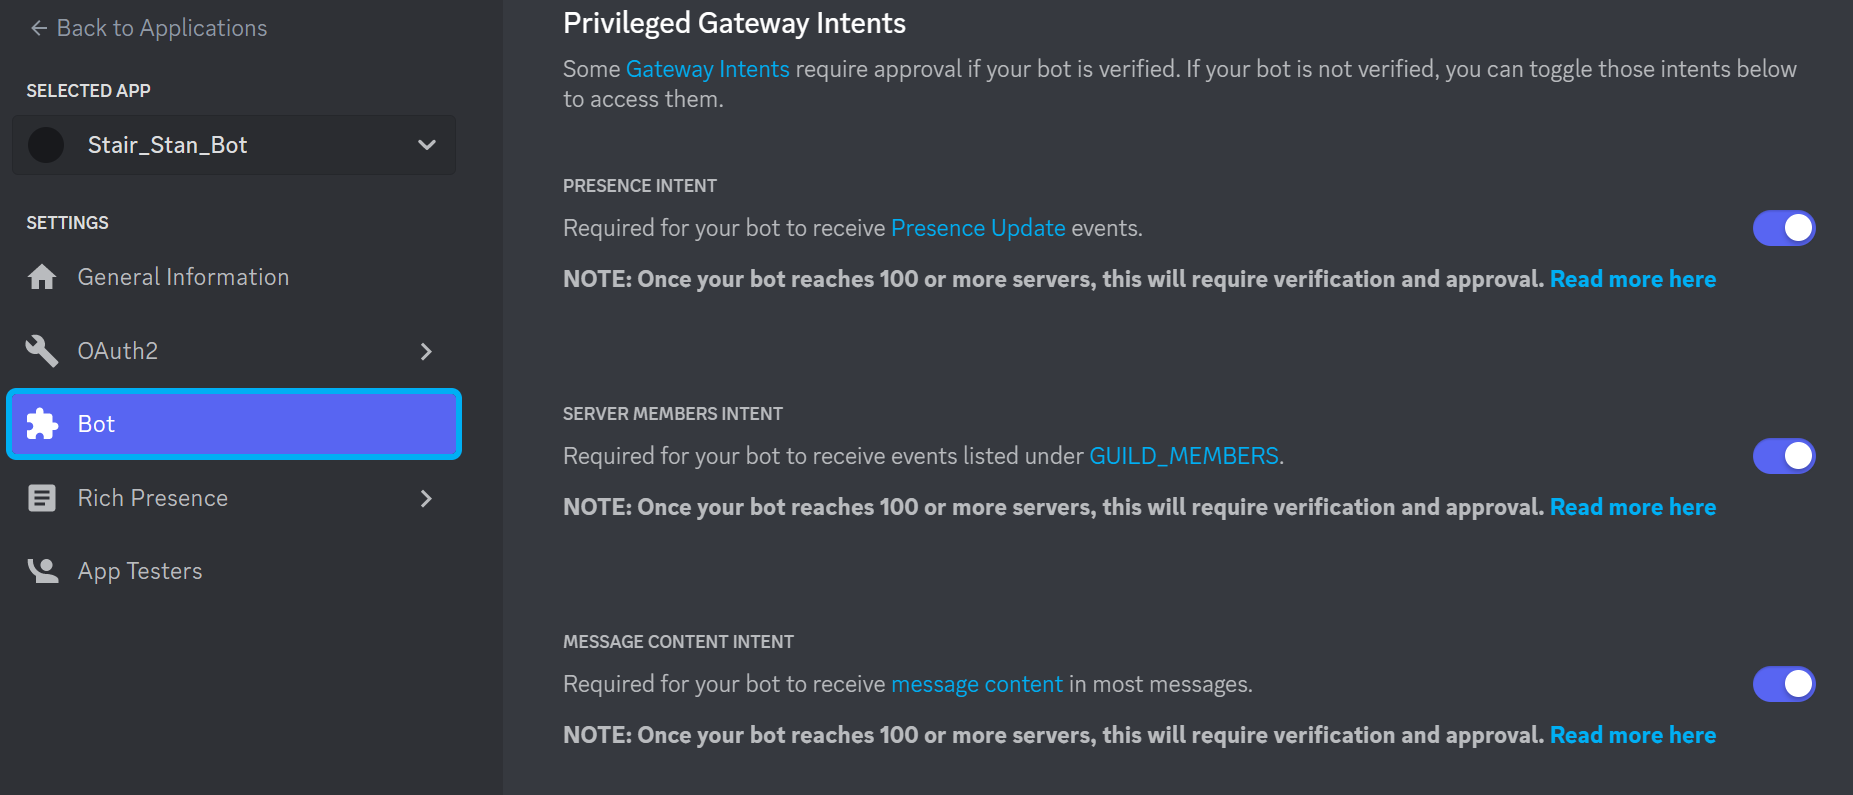
\includegraphics[width=1\textwidth]{img/discord_developer_privileged_intents.png}
    \caption{Privileged Intents für Discord Bot}
    \label{fig:delevoper-privileged-intents}
\end{figure}

Nun können verschiedene Events beim DiscordClient abonniert werden.

\begin{lstlisting}[language=csharp]
// EventHandler.cs
_discordSocketClient.UserJoined += _onUserJoinedEvent.OnUserJoined;
_discordSocketClient.MessageReceived += _messageHandler.OnMessageReceived;
\end{lstlisting}

Es wird für jeden Event eine eigene Klasse erstellt.
So können diese schön gekapselt und seperat behandelt werden.\\
Wie man im Code sehen kann, gibt es für den DiscordSocketClient nur ein MessageReceived Event.
Dieses Event entscheidet noch nicht, ob es sich um eine allgemeine Nachricht im Chat handelt, 
eine Direkte Nachricht an den Bot oder einen Befehl.\\\\
Im Anhang auf Seite \pageref*{fig:message-handling} findet man das Klassendiagramm zum Thema Message Handling.\\\\
Um jetzt nicht alle Nachrichten in einer Klasse bearbeiten zu müssen, wird auf die Hilfe von Interfaces zurückgegriffen.\\
Alle Nachrichten werden an die \textit{MessageHandler} Klasse weitergeleitet.
Dort wird eine Vorselektion gemacht, ob es sich bei den eintreffenden Nachrichten um System Messages handelt, oder um andere Bot Nachrichten.
Wird diese Vorselektion nicht gemacht, kann es sein, dass es zu einer Endlos-Schleife führt, 
da der Bot auch seine eigenen geschriebenen Nachrichten in der \textit{MessageReceived} Methode empfängt.\\
Im Anschluss wird jede Implementation der \textit{IMessageReceiver} Klasse durchgegangen und überprüft,
ob die MessageSource korrekt ist und die \textit{IsMatch} Methode true zurückgibt.
Nur wenn beide Anforderungen erfüllt sind, wird die Nachricht an die jeweilige Message Receiver Implementation weitergeleitet.

\subsubsection*{Das EmailMessageReceivedEvent}
Die \textit{EmailMessageReceivedEvent}-Klasse implementiert das \textit{IMessageReceived}-Interface 
und ist somit ein Empfänger des MessageReceived Events von Discord.
In der \textit{EmailMessageReceivedEvent} Klasse wird eine Nachricht als Direct Message erwartet. 
Sie soll die Form \textit{<vorname.name>@stud.hslu.ch} oder \textit{<vorname.name>@hslu.ch} haben. 
Alle Nachrichten, die nicht diesem Muster entsprechen werden nicht behandelt. 
Dies erlaubt es nur Mitarbeitern oder Studenten der Hochschule sich im Discord Server zu authentifizieren.\\\\
Sobald die Nachricht diesem Muster entspricht, wird sie der \textit{ProcessMessage} Methode übergeben. 
Dort wird zuerst in der Datenbank überprüft ob der Nutzer vorhanden ist. 
Falls nicht, wird eine Fehlermeldung an den Nutzer zurückgegeben. 
Wenn alles stimmt, wird ein Code für die Verifikation generiert.\\ 
Bei der Generierung des Codes wird eine zufällige 6 stellige Zahl erstellt und diese, zusammen mit der Discord Author Id, in einer Liste gespeichert. 
Solange der Server online ist, werden offene Authentifikation in dieser Liste persisitiert. 
Falls der Server aus einem unerklärlichen Grund heruntergefahren wird, oder die Applikation neu gestartet wird, 
muss der Authentifizierungsprozess von neuem begonnen werden.
Dies wird allerdings in Kauf genommen, da noch nichts von Bedeutung für den Benutzer oder den Server passiert ist.\\\\
Sobald der Code generiert wurde, wird dieser, zusammen mit einer Nachricht, dem Benutzer an die angegebene E-Mail Adresse gesendet 
und eine Nachricht an den Benutzer zurückgegeben.\\
Damit ist dieser Schritt abgeschlossen.

\subsubsection*{Das VerificationCodeMessageReceivedEvent}
Die \textit{VerificationCodeMessageReceivedEvent}-Klasse implementiert auch das \textit{IMessageReceived}-Interface.
Damit eine Nachricht an diese Klasse weitergeleitet wird, muss es auch eine Direct Message an den Bot sein, 
swoie eine 6-stellige Zahl. 
Diese Überprüfung wird mit dem Regex-String "\textbf{\^[0-9]\{6\}\$}" erreicht.
Wenn die Nachricht dem korrekten Muster entspricht, wird in der Liste im VerificationCodeManager überprüft, 
ob eine offene Authentifizierung von diesem Nutzer mit diesem Code existiert.
Falls dies nicht der Fall ist, wird eine Fehlermeldung an den Nutzer zurückgegeben.\\\\
Wenn der Code korrekt ist. wird in der Datenbank ein neuer \textbf{DiscordAccount} erstellt.
Dieser wird mit dem zugehörigen Studenten, mithilfe der E-Mail, verbunden.
Des Weiteren wird in der Zwischentabelle \textbf{DiscordAccountDiscordRole} die Verbindung zu den Rollen erstellt.
Für neu authentifizierte Studenten wird die Rolle \textbf{student} und die richtige Haus-Rolle zugewiesen.\\\\
Sobald die Manipulationen auf der Datenbank abgeschlossen sind, werden die Änderungen auch auf den Discord übertragen.
Also der Student bekommt dort vom Bot die Rollen zugewiesen.
Damit hat er jetzt vollen Zugang zum STAIR-Server.\\\\
Im Falle, dass der Benutzer sich schon einmal auf dem STAIR Server authentifiziert hat, 
aber aus irgendeinem Grund den Server verlassen hat, muss er sich noch einmal authentifizieren.
Allerdings werden keine Datenbankmanipulationen gemacht, sondern die Rollen, welcher er ja schon besitzt, zurückgegeben.

\newpage
\subsection{Sprint 3}
In diesem Kapitel wird sich mit der Command Service Architektur von Discord auseinandergesetzt.
Des weiteren wird die Implementation der show- und hide Module- Commands genauer erklärt.

\subsubsection{Command Service Architektur}
Der Command Service wird von Discord verwendet, um Befehle an den Bot zu schicken.
Der Service wird unabhängig neben dem Discord Client gestartet aber nimmt diesen, beim Ausführen der Commands als Kontext entgegen.

\subsubsection*{Starten des Command Service}
Der Command Service wird wie folgt dem Hosting Environment hinzugefügt.

\begin{lstlisting}[language=csharp]
// Program.cs

.AddSingleton(new CommandService(new CommandServiceConfig
    {
        DefaultRunMode = RunMode.Async,
        LogLevel = LogSeverity.Debug
    }))
\end{lstlisting}

Beim Starten des Event Handlers wird der Command Service initialisiert.
Durch die Methode \textbf{AddModulesAsync} geht der Command Service automatisch durch die ganze Projektstruktur durch und 
sucht nach Klassen, welche von \textit{ModuleBase<SocketCommandContext>} erben. 
Diese fügt er dann dem Context, in dem der Bot läuft, hinzu.

\begin{lstlisting}[language=csharp]
// EventHandler.cs

await _commandService.AddModulesAsync(Assembly.GetEntryAssembly(), provider);
\end{lstlisting}

\subsubsection*{Der CommandMessageReceivedEvent}
Die Befehle, welche der Benutzer schicken kann, werden als normale Nachrichten verarbeitet.
Dies bedeutet, dass sie auch durch die \textbf{MessageReceived} Methode abgefangen werden.
In der \textit{CommandMessageReceivedEvent}-Klasse werden alle Nachrichten mit dem Command-Prefix verarbeitet.
Dieser ist in der Config Datei hinterlegt und kann geändert werden.
Für das Projekt wird der Prefix \textbf{!} verwendet.
Falls eine Nachricht mit diesem Prefix eintrifft wird mit folgender Anweisung versucht diesen Befehl auszuführen.

\begin{lstlisting}[language=csharp]
// CommandMessageReceivedEvent.cs

var context = new SocketCommandContext(_discordSocketClient, message);
var result = await _commandService.ExecuteAsync(context, argPos, _serviceProvider);
\end{lstlisting}

Nun schaut der Command Service durch alle Commands durch, 
welche er im vorherigen Schritt mit der \textbf{AddModulesAsync} Methode hinzugefügt hat.
Falls er diesen Command nicht erfolgreich ausführen konnte, gibt er eine Fehlermeldung zurück, 
die wiederum in geigneter Form den Benutzer mitgeteilt wird.

\subsubsection*{Command-Klassen erklärt}
Die Command Klassen erben, wie im vorherigen Kapitel erklärt, von \textbf{ModuleBase<SocketCommandContext>}.
Dudurch werden alle Methoden, welche in der Klasse mit einem \textbf{[Command()]} Attribut versehen sind,
dem Command Service hinzugefügt.

\begin{lstlisting}[language=csharp]
// Miscellaneous.cs

public class Miscellaneous : ModuleBase<SocketCommandContext>
{
    [Command("ping")]
    [Alias("latency")]
    [Summary("Displays the bot's current latency")]
    public Task PingCommand() => ReplyAsync($"Pong! The bot's latency is {Context.Client.Latency} ms.");
}
\end{lstlisting}

Der Text, welcher im Command-Attribut steht, ist der Befehl, den der Benutzer im Discord ausführen muss.
Im obigen Beispiel wäre dies: \textbf{!ping}.\\
Je nach Anwendungsfall können noch weitere Attribute ergänzt werden.
So wird oben ein Alias und eine Beschreibung hinzugefügt.
Es können aber auch Berechtigungsfragen schon mit diesen Rollen abgeklärt werden.
Zum Beispiel gibt es ein \textbf{[RequireRole()]} - Attribut, welches eine bestimmte Rolle zum Ausführen des Commands vorgibt.
Befehle können auch Argumente entgegennehmen.
Diese werden einfach als Argumente im Methodenkopf angegeben.
Falls mehrere Parameter verwendet werden müssen, muss das Attribute \textbf{[Remainder]} hinzugefügt werden.
Dies verhindert, dass nur das letzte Argument an den Bot übertragen wird.\\\\
Der \textbf{Context} wird von ModuleBase geerbt.
Dadurch können der Channel oder der Benutzer, der den Befehl geschickt hat, abgefragt werden.
Dies erweisst sich nützlich, wenn gewisse Befehle nur in gewissen Channeln abgesetzt werden dürfen.\\\\
Für den Anfang wurde ein \textbf{!ping} Befehl und ein \textbf{!help <command>} Befehl hinzugefügt.
Der ping-Befehl gibt die aktuelle Antwortzeit des Bots zurück.
Beim help-Befehl werden alle Commands, welche registriert sind, aufgelistet.
Desweiteren kann auch ein \textbf{!help <command>} Befehl ausgeführt werden, um detailiertere Informationen zu einem Befehl zu erhalten.

\subsubsection{show/hide <module> Command}

Die beiden Commands show und hide können von Studenten benutzt werden um sich selbst an einem Modul Discord Channel hinzuzufügen und sich dann über das Modul austauschen zu können.
Der Name des Moduls muss hierfür spezifisch formatiert sein.
Eine Anleitung hierzu wird dem Studenten auf dem Channel zum Anmelden bei den Modulen angezeigt.
Diese Anleitung wird auch gepinnt, damit sie zwischen den vielen Nachrichten nicht untergeht.

Der angegebene Modulname muss dem Kurznamen entsprechen.
Gross und Kleinschreibung darf ignoriert werden, da im hintergrund dies einheitlich umgewandelt wird.
Einige Module haben am Ende des Kurznamens eine Erweiterung um die verschiedenen Durchführungen, z.B. bei verschiedenen Professoren, zu unterscheiden.
Auch der Prefix und Suffix muss entfernt werden, welche den Studiengang, bzw. das Jahr und Semester beinhaltet.

Beispiele:

% TODO
% \begin{table}[h]
%     \centering
%     \begin{tabular}{|1|p{20em}|1|}
%         \hline
%         \rowcolor[gray]{.9} Angezeigt im MyCampus & Beispiel Befehl & Voller Modulname \\
%         \hline
%         I.BA_GAMEDEV.H2201 & show gamedev & Game Development \\
%         \hline
%     \end{tabular}
%     \caption{Show und Hide Command Beispiele}
%     \label{tab: Show und Hide Command Beispiele}
% \end{table}

Diese Umwandlung muss ebenfalls beim Laden der Modul-Liste des Sekretariats durchgeführt werden.
Diese automatische Umwandlung wurde durch Unit Tests getestet.
Genauere Angaben zu den Tests können im Kapitel \nameref{Testdrehbuch} gefunden werden.
Die Abkürzungen können Studenten über die Modulliste der HSLU herausfinden und wird gleich hinter dem vollen Namen angezeigt.\autocite{noauthor_bachelor_nodate}

\begin{figure}[hb]
    \centering
    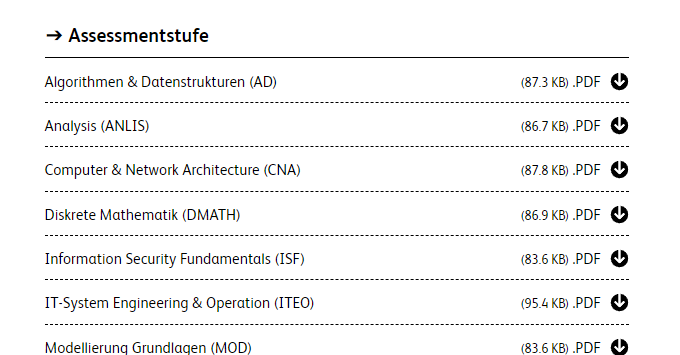
\includegraphics[width=0.8\textwidth]{img/ausschnittModullisteHsluInformatik.PNG}
    \caption{Ausschnitt der Modulliste des Informatik Studiengangs}
    \label{fig:modulliste-informatik}
\end{figure}
\clearpage

\subsubsection{E-Mail Service}
Der E-Mail Service wird im Authentifizierungsprozess benötigt.
Der Benutzer bekommt damit eine E-Mail mit dem Verifizierungscode auf die angegebene Studentenadresse gesendet.
Diesen Code muss er an den Bot zurücksenden um die Authentifizierung abzuschliessen.\\\\
Es wurde über verschiedene Lösungen zu diesem Problem diskutiert.
So könnte man zum Beispiel einen eigenen Mail Server hosten und die Mails über diesen verschicken.
Eine weitere Möglichkeit bestand in der Nutzung des Hochschul-Enterprise-Labs.
Diese bieten einen Mail Dienst an, mit dem man für private Applikationen Mails versenden kann.
Oder man benutzt die bestehende Lösung des alten Stan Bots.\\
Für dieses Projekt wurde entschieden, die bestehende Lösung weiter zu benutzen.
Dies aus dem Grund, da der Mail Service etabliert ist und funktioniert und die Infrastruktur schon besteht.
Für das Team bestand kein Grund diesen zu ersetzten.\\\\
Um Mails aus einer Applikation verschicken zu können, müssen diese über einen Account auf einem Mail Server verschickt werden.
Man muss sich also auf einen Mail Server verbinden, um dort mit einem registrierten E-Mail Account die Mail versenden zu können.
Um dieses Problem zu lösen, wird mit den Angeboten von Microsoft gearbeitet.\\
Als Mail Server wird Outlook verwendet.
Dies aus dem Grund, da alle Studenten ein Microsoft Konto besitzen und ihre E-Mails über Outlook verwalten.
Auch STAIR nutzt Outlook um ihre E-Mails zu versenden.

\subsubsection*{Mircosoft Identity \& Microsoft Azure}
%https://learn.microsoft.com/en-us/azure/active-directory/develop/quickstart-register-app
Die Microsoft Identity Platform erlaubt es Entwicklern einen Authentifizierungsmechanismus in ihre Applikation einzubauen.
Für Besitzer eines Microsoft Azure Administator Kontos oder Office 365 ist die Lösung kostenlos und da auch STAIR einen Office 365 Account hat,
bietet sich diese Lösung an.
Die Microsoft Identity Platform baut auf der OpenId Technologie auf und kann damit jeden OpenId Connect Provider hinzufügen, bzw. diesen nutzen.
Um einer Applikation diese Authentifizierungsmechanismen hinzuzufügen, muss in Microsoft Azure eine Applikation erstellt werden.
Dort können dann Berechtigung für die Benutzer und die Applikation eingestellt werden, sowie die App-Id herausgelesen werden. \autocite{noauthor_introduction_nodate}
Dies sieht man auf folgender Abbildung.

\begin{figure}[h]
    \centering
    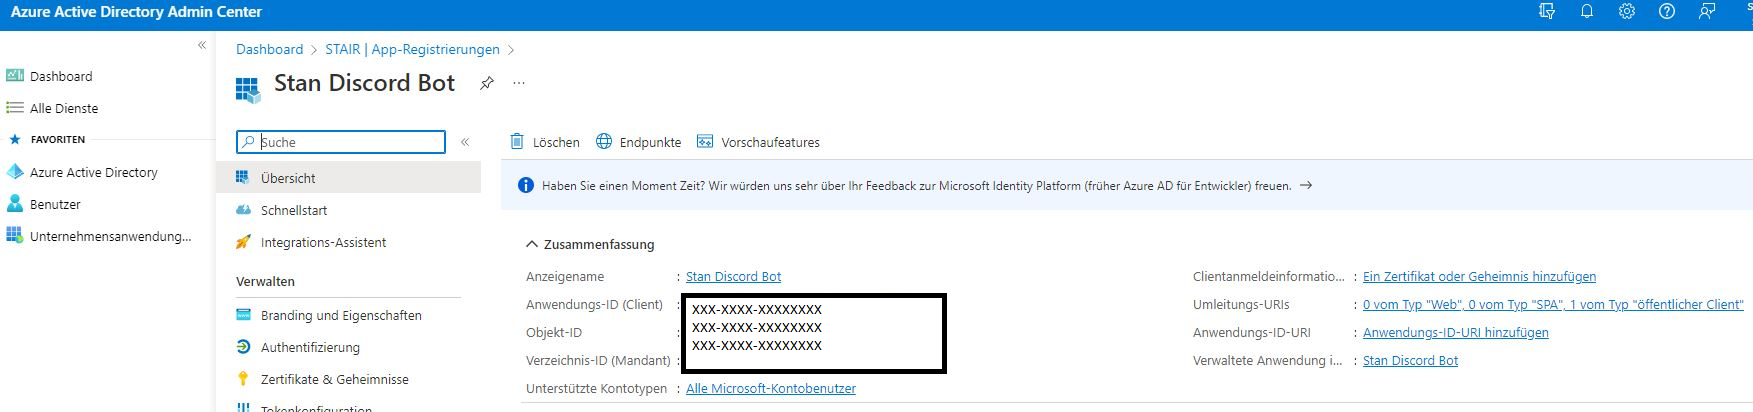
\includegraphics[width=1\textwidth]{img/azure_discord_app_blacked.png}
    \caption{Azure Discord App Registration}
    \label{fig:azure-discord-app-registration}
\end{figure}

Wenn man die Authentifizierungsmöglichkeiten bei der registrierten App aktiviert, wird automatisch Microsoft Identity verwendet.\\\\
Für den Discord Bot wurde von Microsoft Identity die Microsoft Authentication Library (MSAL) benutzt. \autocite{dickson-mwendia_initialize_nodate}
Diese ist Teil von Microsoft Identity.
Damit kann man sich einen Client erstellen, mit dem man sich Authentifizieren kann.

\begin{lstlisting}[language=csharp]
// DeviceCodeAuthProvider.cs
_msalClient = PublicClientApplicationBuilder
                .Create(appId)
                .WithAuthority(AadAuthorityAudience.AzureAdAndPersonalMicrosoftAccount, true)
                .Build();
\end{lstlisting}

Dem \textit{PublicClientApplicationBuilder} kann man die Anwendungs-ID mitgeben, welche man auf der registrierten Azure Applikation auslesen kann.
Im Anschluss wird ausgewählt, wie man sich identifizieren möchte.
Microsoft Identity bietet dort die gängigen Authentifizierungsmöglichkeiten an.
So kann man sich mit dem Microsoft Konto anmelden oder aber über Third-Party Anbindungen authentifizieren.
Dies nennt Microsoft, Hybrid Identity. \autocite{billmath_what_nodate}
Für den Discord Bot wird das Gerät, auf dem die Applikation läuft, beim Starten einmalig authentifiziert und man erhält ein Access Token zurück.
Dieses wird im nächsten Schritt für die Kommunikation mit der Microsoft Graph API verwendet.

\subsubsection*{Microsoft Graph}
Microsft Graph ist eine REST Schnittstelle von Microsft, mit dazugehörigen Clientbibliotheken.
Mit diesen kann man alle Microsoft Service ansprechen. \autocite{angelgolfer-ms_microsoft_nodate}
Diese REST Schnittstelle kann man aus der eigenen Applikation aufrufen, um zum Beispiel über die Azure Applikation eine E-Mail zu versenden.
Microsoft Graph läuft in der Grundlage mit einem Authentifizierten Benutzer oder Gruppen.
So kann man über die REST Schnittstelle, sich zu jeder seiner Microsoft Anwendungen, Daten beschaffen.\\\\
Das Token, welches man von nach der Authentifikation mit Microsoft Identity erhält, kann nun der Klasse \textbf{GraphServiceClient} übergeben werden.
Der GraphServiceClient ist Teil von Microsoft Graph und erlaubt es über die Graph API, REST Endpunkte aufzurufen.
So kann eine Post Request auf den Endpunkt \textit{https://graph.microsoft.com/v1.0/me/sendMail} gesendet werden.
In der Applikation würde der Request wie folgt aussehen.

\begin{lstlisting}[language=csharp]
// MailServicce.cs
await _graphServiceClient.Me.SendMail(message).Request().PostAsync();
\end{lstlisting}

Da der GraphServiceClient mit dem richtigen Microsoft Konto authentifiziert ist, 
werden nun die E-Mails direkt über das richtige Outlook Konto weitergeleitet.

\begin{figure}[h]
    \centering
    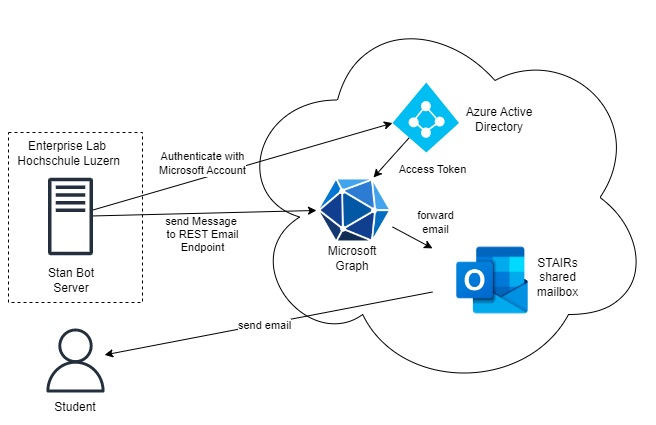
\includegraphics[width=1\textwidth]{img/Email_Infrastruktur.png}
    \caption{Email Versand Infrastruktur}
    \label{fig:send-email-infrastructure}
\end{figure}

\newpage
\subsection{Sprint 4}
In diesem Sprint werden die Statistiken für die STAIR Administration und ihrer Mitglieder implementiert.

\subsubsection{Statistiken}
In den Anforderungen wurde gewünscht, dass man als STAIR Mitglied mithilfe der Datenbank verschiedene Statistiken auslesen kann.
Die Art, wie man diese Statistiken erhält, konnte selbst entschieden werden.
Das Team hat entschieden, diese über Bot Commands zu erstellen.
Mit den Commands ist es möglich, Befehle für den Bot zu übergeben.
Da dieser über das Repository Pattern Zugriff auf die Datenbank hat, kann er die gewünschten Queries absetzten.\\
Eine weitere Möglichkeit wäre gewesen,  Statistiken mithilfe von Scripts abzufragen.
Mit dieser Methode müsste man sich allerdings auf den Server im Enterprise Lab verbinden, die Scripts heraussuchen und diese dort ausführen.
Dies wurde als nicht leicht erweiterbar und benutzerfreundlich eingestuft und aus diesem Grund verworfen.\\\\
Für dieses Projekt wurden 4 verschiedene Statistiken implementiert.
Weitere können aber einfach hinzugefügt werden.\\
Die 4 Statistiken sind:
\begin{itemize}
    \item Anzahl Studenten Pro Haus
    \item Anzahl Studenten pro Semester
    \item Anzahl registrierter Discord Accounts mit Studenten aus jeweiligem Semester
    \item Anzahl Mitglieder pro Modul-Channel
\end{itemize}
Die Befehle werden in Discord wie folgt abgesetzt:
\begin{itemize}
    \item \textbf{!studentsPerHouse}
    \item \textbf{!studentsPerSemester}
    \item \textbf{!accountsPerSemester}
    \item \textbf{!membersPerModule}
\end{itemize}
Die Abfragen werden in den weiteren Kapiteln noch genauer beschrieben.

\subsubsection*{Aufruf Berechtigungen}
Es sollen nur Administratoren und STAIR Mitglieder diese Commands einsehen und ausführen können.
Dazu wurde bei den Commands das Attribute [RequireRole("stair")] und [RequireRole("administrator")] gebraucht.
Diese Attribute haben allerdings nicht funktioniert.
Es konnten immer noch Mitglieder ohne diese Rollen die Commands absetzen.\\
Deshalb wurde eine andere Lösung implementiert.
Auf Discord wird dabei ein \textbf{\#bot-commands} Text-Channel erstellt.
Auf diesen haben nur die Administartoren und STAIR-Mitglieder Zugriff.
Der Bot führt die Befehle jetzt nur aus, wenn Sie von diesem Channel geschickt werden.

\subsubsection*{Plotting Library}
Damit Statistiken einfacher verständlich und aussagekräftig sind, verwendet man Diagramme (engl. Plots).
Plotting Libraries gibt es viele, doch es wurde sich für das kostenlose OpenSource Projekt ScottPlott entschieden.
ScottPlot ist für .NET entwickelt und liefert viele verschiedene Chart-Möglichkeiten, die einfach erstellt und bearbeitet werden können, mit.
Die Verwendung ähnelt sehr der Library Matplotlib und ist dadurch für Personen, die sich schon mit Statistiken im Programmieren beschäftigt haben, einfach zu lernen.
Sie bieten alle bekannten Diagramm-Arten an und erlauben es auch interaktive Plots zu erstellen. \autocite{noauthor_scottplot_nodate}

\newpage
\subsubsection*{Statistik: Students per house}
In dieser Statistik werden die Anzahl Studenten pro Haus zurückgegeben.
Grundlage dafür bietet folgende SQL Query:

\begin{lstlisting}[language=SQL]
SELECT HouseName, Count(s.StudentId) AS StudentCount
FROM students AS s
INNER JOIN houses AS h ON s.FkHouseId=h.HouseId
GROUP BY h.HouseName;
\end{lstlisting}

Übersetzt in eine Linq Query ergibt sich folgendes.

\begin{lstlisting}[language=SQL]
// StudentRepository.cs

from s in db.Student
join h in db.House on s.FkHouseId equals h.HouseId
group s by h.Name into g
select new StudentsPerHouseDTO
{
    HouseName = g.Key,
    StudentsCount = g.Count()
};
\end{lstlisting}

Dargestellt wird diese Abfrage in einem Bar-Plot, wobei die x-Achse die verschiedenen Häuser sind und die y-Achse die Anzahl Studenten in einem Haus.
Die einzelnen Bars werden nach den Farben des Hauses dynamisch eingefärbt.

\begin{figure}[h]
    \centering
    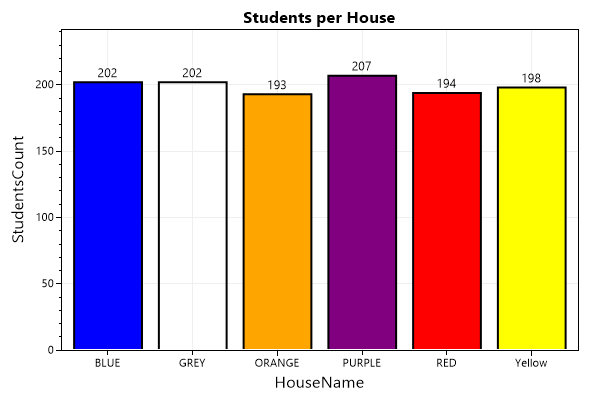
\includegraphics[width=0.8\textwidth]{img/studentsPerHouse.png}
    \caption{Students per house}
    \label{fig:students-per-house}
\end{figure}

\newpage
\subsubsection*{Statistik: Students per semester}
In dieser Statistik werden die Anzahl Studenten in den verschiedenen Semestern zurückgegeben.
Die Anzahl der Semester wird bestimmt, durch die registrierten Studenten, in der Liste der Hochschul Administration.\\
Die grundlegende SQL Query ist folgende:

\begin{lstlisting}[language=SQL]
SELECT Semester, Count(s.StudentId) AS StudentCount
FROM students AS s
GROUP BY s.Semester;
\end{lstlisting}

Übersetzt als Linq Query ergibt sich folgendes.

\begin{lstlisting}[language=SQL]
// StudentRepository.cs

from s in db.Student
group s by s.Semester into g
select new StudentsPerSemesterDTO
{
    Semester = g.Key,
    StudentsCount = g.Count()
};
\end{lstlisting}

Die Abfrage wird als Bar-Plot dargestellt. 
Auf der x-Achse befinden sich die verschiedenen Semester und auf der y-Achse die Anzahl der sich darin befindenden Studenten.

\begin{figure}[h]
    \centering
    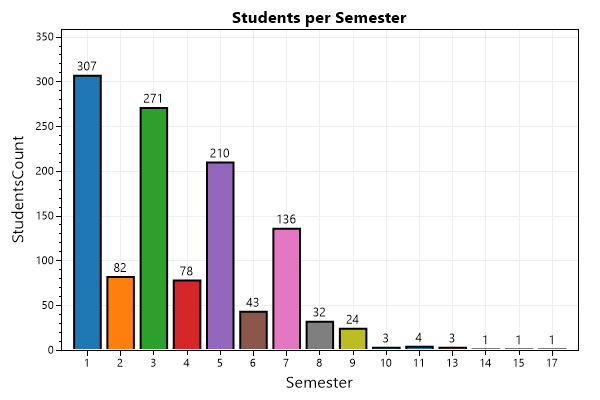
\includegraphics[width=0.8\textwidth]{img/studentsPerSemester.png}
    \caption{Students per semester}
    \label{fig:students-per-semester}
\end{figure}

\newpage
\subsubsection*{Statistik: Accounts per semester}
In dieser Statistik kann die Anzahl, der sich im STAIR Discord Server authentifizierten Personen, abgefragt werden.
Gruppiert wird dabei wieder nach dem Semester in dem sich der Student befindet.
So kann herausgefunden werden, in welchen Semestern sich die Discord Benutzer durchschnittlich befinden.
Die grundlegende SQL Query ist folgende:

\begin{lstlisting}[language=SQL]
SELECT s.Semester, Count(ac.FkStudentId)
FROM discordaccounts AS ac
RIGHT JOIN students AS s ON ac.FkStudentId=s.StudentId
GROUP BY s.Semester;
\end{lstlisting}

Diese Query ist etwas schwieriger in Linq zu übersetzten, da es so etwas wie \textbf{RIGHT JOIN} in Linq nicht gibt.
Stattdessen müssen die Aufrufe der Tabellen in der Query vertauscht werden.
Also die Tabelle, welche man mit \textbf{RIGHT JOIN} ganz anzeigen möchte, muss zuerst selektiert werden.
Im Anschluss wird dann die andere gejoint.\\
Damit auch leere Felder anzeigt werden, also z.B. Semester in denen es keine registrierten Studenten hat, 
muss der Befehl \textit{DefaultIfEmpty()} auf der gejointen Gruppe aufgerufen werden.

\begin{lstlisting}[language=SQL]
// DiscordAccountRepository.cs

from s in db.Student
join dc in db.DiscordAccount on s.StudentId equals dc.FkStudentId into joinGroup
from gr in joinGroup.DefaultIfEmpty()
group gr by s.Semester into g
select new DiscordAccountsPerSemesterDTO
{
    Semester = g.Key,
    AccountsCount = g.Count(stud => stud.FkStudentId != null)
};
\end{lstlisting}

Diese Abfrage wird, gleich wie die vorherige, auch als Bar-Plot dargestellt. 
Auf der x-Achse befinden sich die verschiedenen Semester und auf der y-Achse die Anzahl der authentifizierten Studenten.

\begin{figure}[h]
    \centering
    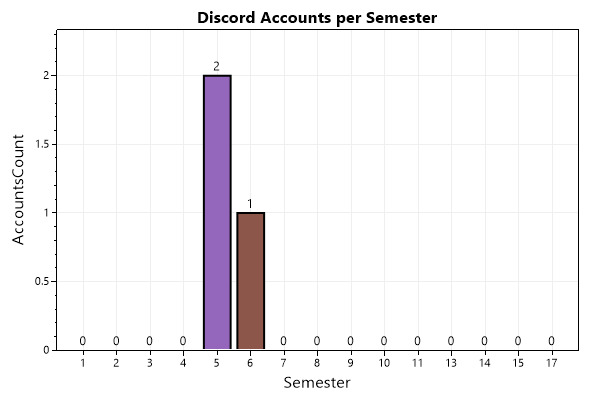
\includegraphics[width=0.6\textwidth]{img/accountsPerSemester.png}
    \caption{Accounts per semester}
    \label{fig:accounts-per-semester}
\end{figure}

\clearpage
\subsubsection*{Statistik: Members per module}
In dieser Statistik können die meist abonnierten Modul Channels abgefragt werden.
Es wird also nach den meisten Mitgliedern sortiert. 
Die Anzahl der Module, die im Chart angezeigt werden sollen, ist über einen Parameter nach dem Befehl einstellbar.
Standardmässig ist die Anzahl Module auf 10 eingestellt.\\
Die grundlegende SQL Query ist folgende:

\begin{lstlisting}[language=SQL]
SELECT m.ChannelName, Count(am.FkDiscordAccountId) AS MemberCount
FROM discordaccountsmodules AS am 
INNER JOIN modules AS m ON am.FkModuleId=m.ModuleId
GROUP BY m.ChannelName
ORDER BY MemberCount DESC;
\end{lstlisting}

Übersetzt als Linq Query ergibt sich folgendes.

\begin{lstlisting}[language=SQL]
// DiscordAccountModuleRepository.cs

from am in db.DiscordAccountModule
join m in db.Module on am.FkModuleId equals m.ModuleId
group m by m.ChannelName into g
orderby g.Count() descending
select new MembersPerModuleDTO
{
    ModuleName = g.Key,
    MemberCount = g.Count()
};
\end{lstlisting}

Diese Abfrage wird als Kuchen-Diagramm dargestellt. So können die Proportionen der einzelnen Module besser erahnt werden.
Die Anzahl der Mitglieder dieser Channels, wird in den Kuchenstücken angezeigt.
Die Legende rechts bietet eine Übersicht der dargestellten Module.

\begin{figure}[h]
    \centering
    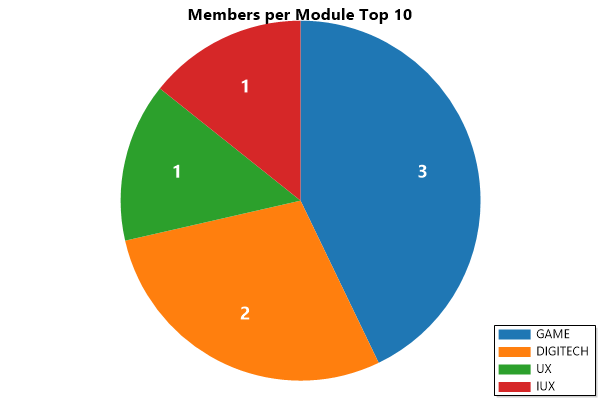
\includegraphics[width=0.7\textwidth]{img/membersPerModule.png}
    \caption{Members per module}
    \label{fig:members-per-module}
\end{figure}
\clearpage

\subsubsection{Logging}
Für ein sauberes Entwickeln und einen sauberen operativen Einsatz gehört das Schreiben von Log-Einträgen dazu.
Damit man nachvollziehen kann, welche Schritte der Bot unternommen hat, sowie bei Fehlern schneller darauf reagieren kann.\\
Als Logging Framework wurde sich für NLog entschieden.\autocite{noauthor_nlog_nodate}
Dies aus dem Grund, da es das verbreiteste Logging Framework für .Net Applikationen ist und es einfach in das Microsoft Logging System integriert werden kann.
Auch ist es Open Source und Frei für die Benutzung.
Für eine saubere Ausführung benötigt NLog eine Konfigurationsdatei.
In dieser kann das Logging Format angegeben werden, die Dateien in welche geloggt werden soll, sowie allfällige Farbeinstellungen für verschiedene Log-Levels.
Die NLog.config Datei für dieses Projekt sieht folgendermassen aus.

\begin{lstlisting}[language=XML]
<?xml version="1.0" encoding="utf-8" ?>
<nlog xmlns="http://www.nlog-project.org/schemas/NLog.xsd" xmlns:xsi="http://www.w3.org/2001/XMLSchema-instance">
    <targets>
        <target name="coloredConsole" xsi:type="ColoredConsole" useDefaultRowHighlightingRules="false"
        layout="${longdate}| ${pad:padding=5:inner=${level:uppercase=true}}| ${pad:padding=-50:inner=${logger}}| ${message:withexception=true}" >
            <highlight-word condition="level == LogLevel.Debug" foregroundColor="Gray" text="DEBUG"/>
            <highlight-word condition="level == LogLevel.Info" foregroundColor="Green" text="INFO" />
            <highlight-word condition="level == LogLevel.Warn" foregroundColor="Yellow" text="WARN" />
            <highlight-word condition="level == LogLevel.Error" foregroundColor="Red" text="ERROR"/>
            <highlight-word condition="level == LogLevel.Fatal" foregroundColor="Red" text="FATAL" backgroundColor="White" />
        </target>
    </targets>
    <rules>
        <logger name="*" minlevel="Debug" writeTo="coloredConsole" />
    </rules>
</nlog>
\end{lstlisting}

Es wurde dabei entschieden nur in die Konsole zu loggen.
Da der Server auf welchem der Bot läuft, wenn es gut läuft, nur einmal im Semester geöffnet werden muss,
wird nicht unnötig Speicherplatz verbraucht.
Die Log Daten kann man sich auch auf der Konsole anzeigen lassen.\\
EIn Log Eintrag sieht dabei wie folgt aus:
\begin{figure}[h]
    \centering
    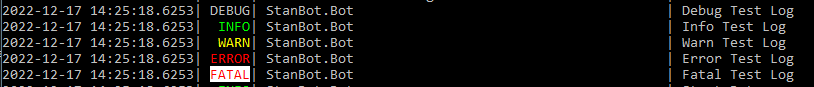
\includegraphics[width=1\textwidth]{img/LogLevels.png}
    \caption{Logging Beispiele}
    \label{fig:logging-examples}
\end{figure}

\newpage
\subsection{Sprint 5}
Im letzten Sprint wird eine Fehler Mitteilung eingebaut, welche einen Admin bei einem Problem informiert.
Auch wird der Bot startbereit gemacht, um ihn auf die produktive Umgebung zu deployen und ein Profilbild erstellt, 
welches ihn als Bot zu erkennen gibt.

\subsubsection{Stan Logo}
Damit der Bot ein sauberes Erscheinungsbild hat, wird für Ihn ein Logo erstellt.
Da Stan schon als Maskottchen von STAIR etabliert ist, nämlich als kleiner Kaktus, 
soll er noch mit einen spezifischen Discord Look ausgestattet werden.\\
Die Designs werden bei STAIR über die Plattform \textbf{Canva} verwaltet und erstellt. \autocite{noauthor_kostenloses_nodate}
Darin wurde auch das Discord Stan Logo geboren.

\begin{figure}[h]
    \begin{minipage}[t]{0.5\textwidth}
        
\includegraphics[width=0.7\textwidth]{img/StanDiscordLogoSolo.png}
    \end{minipage}
    \begin{minipage}[t]{0.5\textwidth}
        
\includegraphics[width=0.7\textwidth]{img/StanDiscordLogo.png}
    \end{minipage}
    \caption{Stan Discord Logo}
    \label{fig:stan-discord-logo}
\end{figure}

Diese Bilder können nun als Profilbild des Bots dienen, sowie als Vermarktungslogo für den STAIR Discord.

\subsubsection{Fehler Mitteilung}
Falls während der Laufzeit Fehler auftreten, also aus irgend einem Grund der E-Mail Service nicht mehr funktioniert, 
oder die Datenbank abstürtzt, soll ein Administrator kontaktiert werden.
Dieser Kontakt soll bei einem Datenbank Absturz über E-Mail erfolgen und bei einem E-Mail Service Absturz über eine private Nachricht auf Discord.\\
Damit der Administrator bei einem Absturz nicht mit Nachrichten und E-Mails überhäuft wird, 
wird der selbe Fehler maximal einmal alle 4 Stunden an den Adminsitrator gesendet.
Das heisst, er bekommt nur einmal die Nachricht eines Absturzes und erst, wenn er das Problem nach 4 Stunden nicht gelöst hat, 
bekommt er wieder eine Nachricht.
\newpage
Damit der Bot weiss, welche Personen als Administrator hinterlegt sind, 
wird in der Datenbank in der Studenten Tabelle das Feld \textbf{IsDiscordAdmin} auf \textbf{True} gesetzt.
Diese Zuweisung zum Discord Administrator kann per Command vorgenommen werden.
Die Commands lauten:
\begin{itemize}
    \item \textbf{!addAdmin} <email-address>
    \item \textbf{!removeAdmin} <email-address>
\end{itemize}
Damit bei einem Datenbank Absturz die Adminstratoren, trotzdem noch ausgelesen werden können, 
werden diese E-Mail Adressen zusätzlich noch in eine Datei \textbf{discordAdmins.csv} gespeichert.
Dies erfolgt auch bei der Ausführung der Commands.\\\\
In den Nachrichten werden folgende Informationen mitgegeben.
\begin{itemize}
    \item Die Art der Nachricht. Also ob es sich um einen Datenbank Fehler oder um einen Fehler des E-Mail Service handelt.
    \item Der Stacktrace der Exception.
    \item Die Message der Exception.
    \item Die Klasse, in welcher der Fehler geworfen wurde.
\end{itemize}
So eine Nachricht kann als E-Mail und als Discord Nachricht folgendermassen aussehen.
\begin{figure}[h]
    \begin{minipage}[t]{0.5\textwidth}
        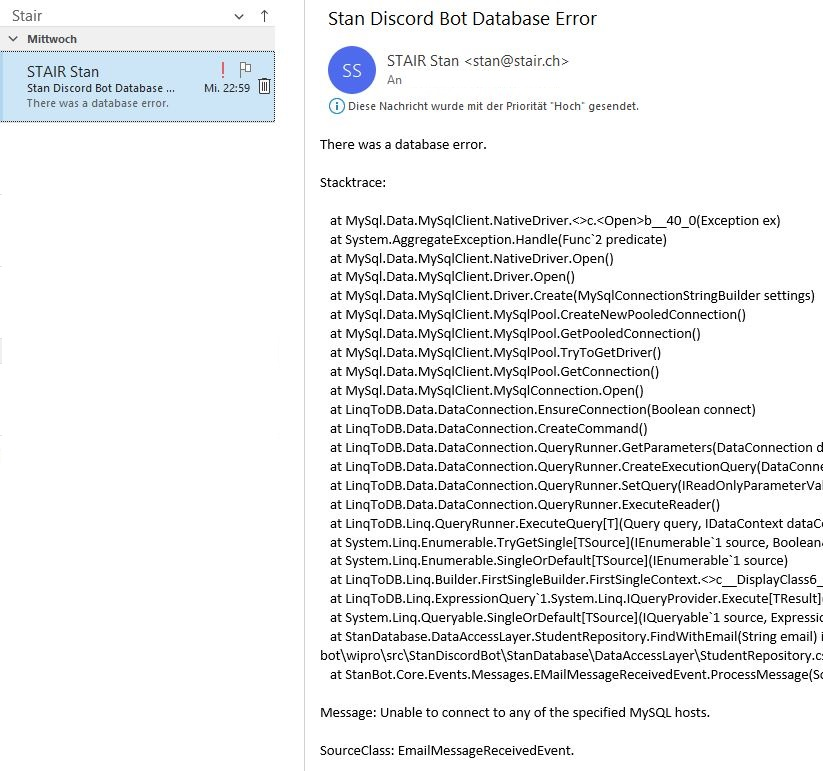
\includegraphics[width=1\textwidth]{img/DatabaseErrorNotificationEmail.png}
        \caption{Fehler Nachricht E-Mail}
    \end{minipage}
    \begin{minipage}[t]{0.5\textwidth}
        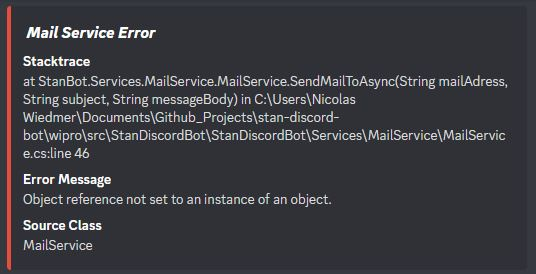
\includegraphics[width=1\textwidth]{img/MailErrorNotificationEmbed.png}
        \caption{Fehler Nachricht Discord}
    \end{minipage}
    \label{fig:error-notifications}
\end{figure}

\subsubsection{Bot als Deamon}
Der Discord Bot wird auf einem Linux Server des Enterprise Labs der Hochschule Luzern deployed.
Dieser soll als Deamon laufen, also als Hintergundservice des Servers.
Mit diesem Vorgehen kann sichergestellt werden, dass der Service ununterbrochen läuft.\\
Um das Deployment auf Linux einfacher zu gestalten, bietet Microsoft auch eine systemd Blibliothek an, 
mit der der Host Provider in diese Umgebung eingefügt werden kann.\autocite{dotnet-bot_systemdhostbuilderextensionsusesystemdihostbuilder_nodate}
Dies kann mit folgendem Code hinzugefügt werden.

\begin{lstlisting}[language=csharp]
\\Program.cs
using IHost host = Host.CreateDefaultBuilder()
                .UseSystemd()
                .ConfigureServices((_, services) => services
                ...)
\end{lstlisting}

Die Bibliothek konfiguriert das Loggen in die Konsole im systems-Format und stellt Benachrichtigungen beim Starten und Beenden der Anwendung bereit.

\newpage
\subsection{Deployment des Bots auf den Linux Server}

\todo{Yannis}

\newpage
\subsection{Testsdurchführung}
\todo{Nicolas}

\newpage
\subsection{Einführung des neuen Bots}
\todo{Yannis}
Es wurde zusammen mit dem STAIR Präsidenten besprochen, dass das Einführen nicht in einem laufenden Semester oder während der Prüfungsphase passiert.
So soll verhindert werden, dass bei einem auftauchenden Bug nicht den Studierenden die Austauschmöglichkeit des Discord Servers genommen wird.

\newpage
\subsubsection{Authentifizierung}
\todo{Nicolas}

\newpage
\section{Evaluation und Validation}

\todo{schreiben}

\subsection{Fehlererkennung}

\section{Ausblick}

\todo{schreiben}

\newpage

\section{Anh\"ange}

\subsection{Sprintreviews}\label{Sprintreviews}
In diesem Kapitel werden die einzelnen Sprintreviews aufgelistet.
Diese beinhalten immer eine Reflektion zum letzten Sprint mit einer Übersicht der umgesetzten User-Stories und
einer Retrospektive über aufgefallenen Problemen und dazugehörigen Massnahmen.

\subsubsection{Sprint 1}
\subsubsection*{Sprintziel}
Studentenerfassung ist implementiert.

\subsubsection*{Risiko-Update}
\begin{itemize}
    \item Kommunikation in Richtung Discord wurde im Vorfeld noch nicht bedacht.
    Kann sein das die Architektur angepasst werden muss, um Kommunikation ausgehend vom Bot starten zu können.
\end{itemize}

\subsubsection*{Sprintbacklog}
In diesem Sprint wurde nur eine User-Story umgesetzt.\\
\url{https://github.com/stairch/stan-discord-bot/issues/2}
\newline
Geschätzer Aufwand: 8h
\newline
Effektiver Aufwand: 6 1/2 h

\subsubsection*{Retrospektive}
Erfolge:
\begin{itemize}
    \item LoadStudenten Script konnte einfach und schnell erstellt werden.
    \item Library Linq2db einfacher als erwartet.
\end{itemize}
Probleme:
\begin{itemize}
    \item Linq2db stellt keine Generierung der Datenbank aus den Klassen zur Verfügung.
\end{itemize}
Massnahmen:
\begin{itemize}
    \item Datenbank Schema muss manuell erstellt werden.
\end{itemize}
\newpage

\subsubsection{Sprint 2}
\subsubsection*{Sprintziel}
Modulerfassung ist implementiert und die Kommunikation mit Discord und dem Bot funktioniert.

\subsubsection*{Risiko-Update}
\begin{itemize}
    \item Keine.
\end{itemize}

\subsubsection*{Sprintbacklog}
In diesem Sprint wurden zwei User-Stories umgesetzt.\\
\url{https://github.com/stairch/stan-discord-bot/issues?q=is%3Aopen+is%3Aissue+milestone%3A%22Sprint+2%22}
\newline
Geschätzer Aufwand: 15h
\newline
Effektiver Aufwand: 16 h

\subsubsection*{Retrospektive}
Erfolge:
\begin{itemize}
    \item Kommunikation mit Discord und dem Bot konnte sichergestellt werden.
    \item Ein Help und ein Ping Befehl konnten zum Testen implementiert werden.
    \item Der Bot schreibt einen Benutzer direkt an, sobald dieser den Server betritt.
    \item Die Modulerfassung alleine funktioniert.
\end{itemize}
Probleme:
\begin{itemize}
    \item Bei der Modulerfassung können die Kategorien noch nicht richtig erstellt werden und zugewiesen werden.
    Die ID der neu erstellten Kategorie wird nicht richtig zurückgegeben.
\end{itemize}
Massnahmen:
\begin{itemize}
    \item Kleines Test Projekt erstellen und weiter versuchen. Auf Logik-Fehler nochmal kontrollieren.
\end{itemize}
\newpage

\subsubsection{Sprint 3}
\subsubsection*{Sprintziel}
Der show/hide <module> Command wurde implementiert und der E-Mail versandt für das Authentifizieren.

\subsubsection*{Risiko-Update}
\begin{itemize}
    \item Die Modulerfassung funktioniert immer noch nicht.
    Prioritäten müssen gesetzt werden.
    Kann sein, dass sich Issues nach hinten verschieben.
\end{itemize}

\subsubsection*{Sprintbacklog}
In diesem Sprint wurden zwei User-Stories umgesetzt.\\
\url{https://github.com/stairch/stan-discord-bot/issues?q=is%3Aopen+is%3Aissue+milestone%3A%22Sprint+3%22}
\newline
Geschätzer Aufwand: 10h
\newline
Effektiver Aufwand: 9 1/2 h

\subsubsection*{Retrospektive}
Erfolge:
\begin{itemize}
    \item Der E-Mail Versand konnte implementiert werden und sollte funktionieren.
    Das Device, auf welchem der Bot läuft, wird beim Starten von dem Azure Dienst erkannt und kann hinzugefügt werden.
\end{itemize}
Probleme:
\begin{itemize}
    \item Der E-Mail versandt läuft über eine Azure Applikation, für die wir die Berechtigung noch nicht haben.
    Das Device kann somit noch nicht hinzugefügt werden.
    \item Die Modulerfassung funktioniert immer noch nicht.
    \item Mit dem show/hide <module> Issue wurde noch nicht begonnen.
\end{itemize}
Massnahmen:
\begin{itemize}
    \item Prioritäten setzten was die Modulerfassung anbelangt.
    \item Möglichst zeitnah mit dem neuen Issue beginnen.
\end{itemize}

\newpage
\subsubsection{Sprint 4}
\subsubsection*{Sprintziel}
Die Statistiken für die STAIR Mitglieder wurden implementiert, sowie ein stabiles Logging Framework.

\subsubsection*{Risiko-Update}
\begin{itemize}
    \item Keine.
\end{itemize}

\subsubsection*{Sprintbacklog}
In diesem Sprint wurde eine User-Story umgesetzt.\\
\url{https://github.com/stairch/stan-discord-bot/issues?q=is%3Aissue+milestone%3A%22Sprint+4%22+}
\newline
Geschätzer Aufwand: 5h
\newline
Effektiver Aufwand: 6 h

\subsubsection*{Retrospektive}
Erfolge:
\begin{itemize}
    \item Das Problem der letzten beiden Sprints mit der Datenbank konnte gelöst werden.
    Dort wurde für die erstellung von Models Konstruktoren eingesetzt.
    Diese wurden allerdings vpn Linq2DB nicht richtig aufgerufen, bzw. befüllt.
    Aus diesem Grund haben wir die Konstruktoren weggelassen und eine statische CreateNew Methode hinzugefügt.
    \item Die Statistiken konnten erfolgreich implementiert werden.
    \item Es konnte ein stabiles Logging Frameworjk NLog in das System eingebunden werden.
    \item Für den E-Mail Versand wurde der richtige Account von STAIR freigeschalten.
    Dieser kann jetzt erfolgreich genutzt werden.
    \item Der show und hide Command konnte erfolgreich umgesetzt werden.
\end{itemize}
Probleme:
\begin{itemize}
    \item Bei den Commands gibt es ein RequireRole Attribut, welches man eigentlich verwenden kann um die Rolle des Aufrufenden Benutzers zu prüfen.
    Dieses funktioniert allerdings nicht.
\end{itemize}
Massnahmen:
\begin{itemize}
    \item Es muss eine Alternative gesucht werden um die Berechtigung einzuholen.
    Man kann z.B. nur von einem bestimmten Channel aus Commands versenden.
\end{itemize}

\newpage
\subsubsection{Sprint 5}
\subsubsection*{Sprintziel}
Die Fehlermeldung wurde im Bot integriert und der Startkonfiguration wurde systemd hinzugefügt.

\subsubsection*{Risiko-Update}
\begin{itemize}
    \item Keine.
\end{itemize}

\subsubsection*{Sprintbacklog}
In diesem Sprint wurde eine User-Story umgesetzt.\\
\url{https://github.com/stairch/stan-discord-bot/issues?q=is%3Aissue+milestone%3A%22Sprint+5%22+}
\newline
Geschätzer Aufwand: 4h
\newline
Effektiver Aufwand: 3 1/2 h

\subsubsection*{Retrospektive}
Erfolge:
\begin{itemize}
    \item Die Fehlermitteilungen konnten erfolgreich hinzugefügt werden.
    \item Die systemd Konfiguration konnte hinzugefügt werden.
    \item Es wurde ein Stan Discord Logo designed und implementiert.
\end{itemize}
Probleme:
\begin{itemize}
    \item Bei immer mehr Klassen in der Dependency Injection, kann es zu Circular Dependencies kommen.
\end{itemize}
Massnahmen:
\todo{Ist Item 4 gewollt? Wurde nicht fertig geschrieben}
\begin{itemize}
    \item Prioritäten setzten was die Modulerfassung anbelangt.
    \item Möglichst zeitnah mit dem neuen Issue beginnen.
    \item Es sollten keine separaten Dokumente, wie Protokolle erstellt werden, sondern man sollte diese direkt einfügen in der Dokumentation um sich das Zusammenführen später zu ersparen.
    \item Dort Clean Coding Vorgehen anwenden. wo es Sinn macht.
    \item Bei immer mehr werdenden Klassen muss informiert werden, wie diese schön ins System injected werden können.
\end{itemize}

\subsection{Diagramme}
\begin{landscape}
    \begin{figure}[hb]
        \centering
        \hspace*{-4.5cm}
        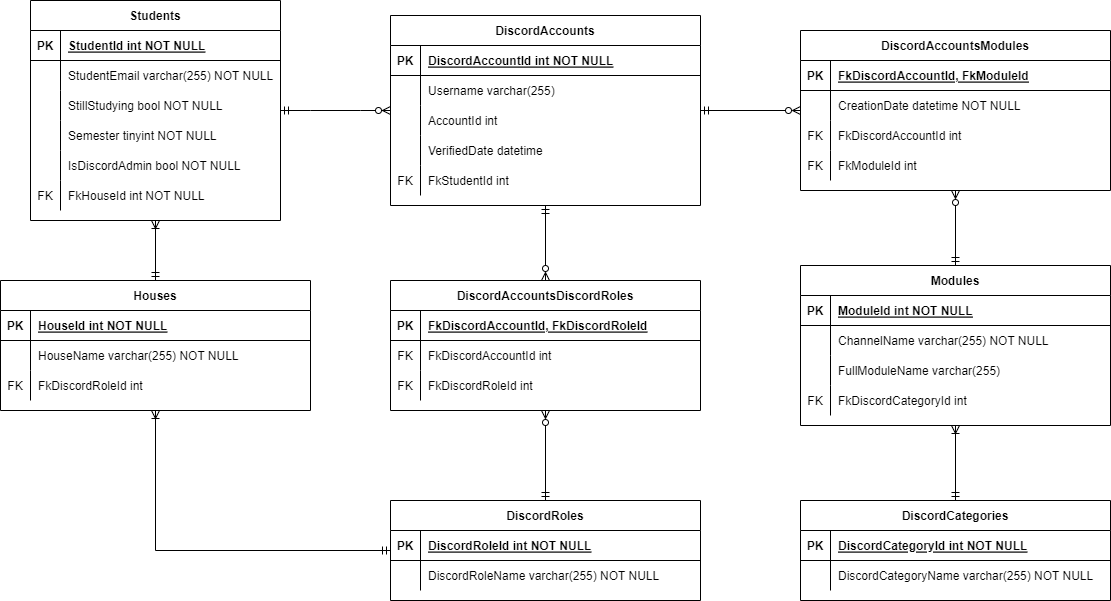
\includegraphics[width=1.6\textwidth]{img/ER-Diagramm.png}
        \caption{Entity Relationship Diagram Gross}
        \label{fig:ER-Diagram-big}
    \end{figure}
\end{landscape}

\begin{figure}[ht]
    \centering
    \hspace*{-2cm}
    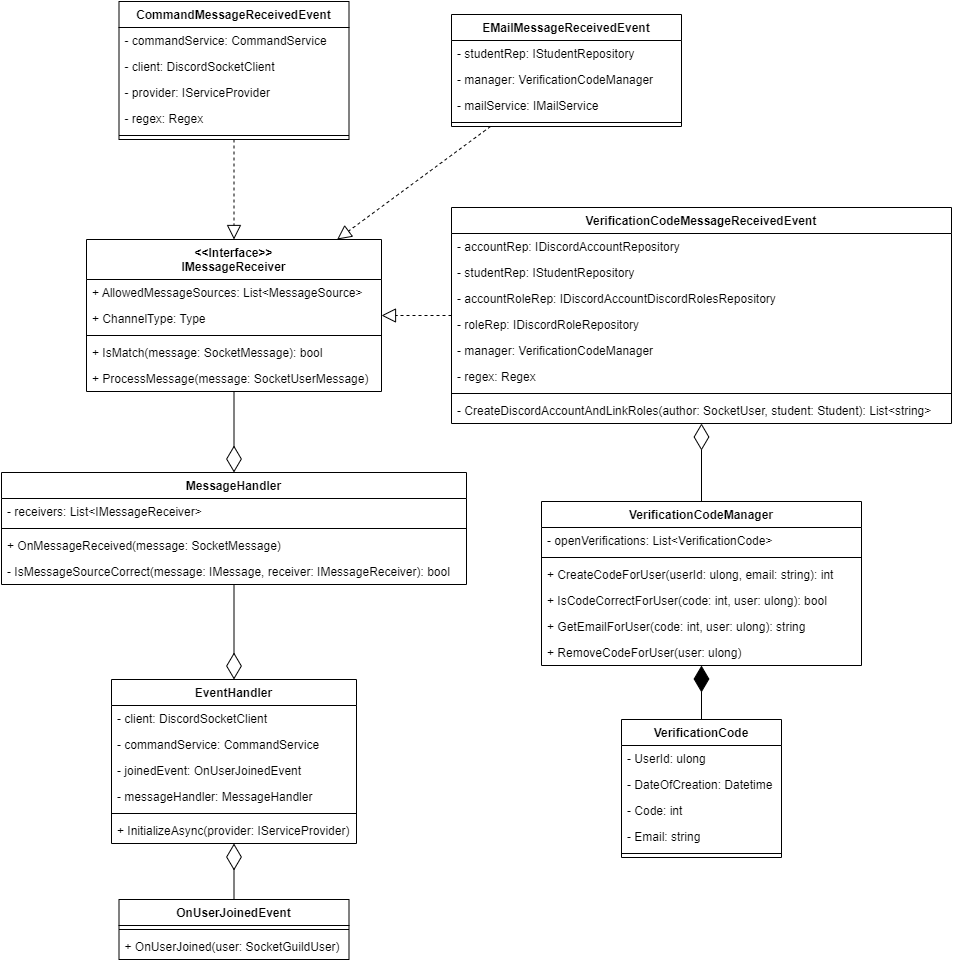
\includegraphics[width=1.3\textwidth]{img/MessageHandling.png}
    \caption{Message Handling}
    \label{fig:message-handling}
\end{figure}
\clearpage

\newpage
\section{Glossar}

API
bzw.
CSV
Deployment
Discord
HSLU
ISA Module
Konsolenanwendungen
REST
z.B.

% https://blog.aristolo.com/de/definition-begriffe-bachelorarbeit-masterarbeit-dissertation/
\todo{schreiben}

\section{Abbildungsverzeichnis}
\listoffigures

\section{Tabellenverzeichnis}
\listoftables

\section{Literaturverzeichnis}
\printbibliography

\newpage
\section{Bedienungsanleitung}\label{Bedienungsanleitung}

\subsection{Aufsetzen des Servers}

Der Stan Discord Bot kann auf verschiedenen Betriebssystemen genützt werden.
In dieser Anleitung wird das Aufsetzen für Ubuntu Linux 20.04 gezeigt.

\todo{Complete tutorial}

\begin{enumerate}
    \item Verbinde zum VPN oder verbinde zum WLAN an der Hochschule
    \item Verbinde zum Server über SSH
        \begin{verbatim}
            $ ssh localadmin@stair-bot-lnx.el.eee.intern
        \end{verbatim}
    \item Führe Updates durch
        \begin{verbatim}
            # sudo apt update
            $ apt list --upgradable
            # sudo apt upgrade -y
            # sudo apt autoremove
        \end{verbatim}
    \item Installiere MySQL
        \begin{verbatim}
            # sudo apt install mysql-server
            # sudo systemctl start mysql.service
        \end{verbatim}
    \item Installiere .NET 6
        \begin{verbatim}
            # wget https://packages.microsoft.com/config/ubuntu/20.04/packages-microsoft-prod.deb -O packages-microsoft-prod.deb
            # sudo dpkg -i packages-microsoft-prod.deb
            $ rm packages-microsoft-prod.deb
            # sudo apt update
            # sudo apt install -y dotnet-sdk-6.0
        \end{verbatim}
    \item Lade den Code auf den Server
        \begin{verbatim}
            # 
        \end{verbatim}
    \item Erstelle die Datenbank
        \begin{verbatim}
            # 
        \end{verbatim}
    \item Starte die Software
        \begin{verbatim}
            # sudo apt update
            # sudo apt upgrade -y
        \end{verbatim}
\end{enumerate}

\subsection{Konfiguration des StanBots}\label{konfigurationStanBot}

Die Settings Datei heisst \textit{stan.json}
\begin{lstlisting}[language=json]
{
    "DisordApplicationToken": "XXXX-XXXXX-XXXXXXXXXXXX",
    "Prefix": "!",
    "GuildId": "1234567891234567",
    "FromEmailAddress": "stan@stair.ch",
    "FromEmailName: "STAN",
    "AppId": "XXXXXXXX-XXXX-XXXX-XXXX-XXXXXXXX",
    "Scopes" ["Mail.Send", "Mail.Send.Shared"],
}
\end{lstlisting}

\subsection{Unterhalt}

Einmal pro Semester müssen die Module und die Studierenden aktualisiert werden.
\todo{Write tutorial}

\subsection{Studenten Liste laden}

Hier wird ein Beispiel dieser Datei gezeigt:

\todo{Add CSV data here}

\todo{Yannis}

%\begin{lstlisting}[language=csv]

%\end{lstlisting}

\subsection{Instandhaltung Stan Discord Bot}

Die Datenbank muss vor jedem Semesterbeginn aktualisiert werden mit der aktuellen Modulliste und der aktuellen Studierendenliste.
Bei der Modulliste ist zu beachten, dass alle Module in der Liste enthalten sein müssen, auch wenn sie dieses Semester nicht durchgeführt werden.
Ansonsten werden bisherige Chatverläufe von Modulen gelöscht, auch wenn diese ein Semester später erneut durchgeführt werden.
Der STAIR Vorstand muss in regelmässigen Abständen die Hilfschannel auf dem Discord Server überwachen um zeitnah den Studierenden helfen zu können.

\subsubsection{Aktualisieren des Servers}

\todo{Yannis}

\subsubsection{Aktualisieren der Module}

\todo{Yannis}

\subsubsection{Aktualisieren der Studierenden}

\todo{Yannis}

\section{Besprechungsprotokolle}

\subsection{Kick Off Meeting 23.09.2022}

\subsubsection*{Anwesende Personen}

\begin{itemize}
    \item Markus Waldmann (WIPRO Betreuer, Dozent)
    \item Nicolas Wiedmer (WIPRO Arbeiter, Student)
    \item Yannis Krämer (WIPRO Arbeiter, Student)
    \item Martin Steiger (STAIR Präsident)
    \item Estefania Otero (STAIR Expräsidentin)
\end{itemize}

\subsubsection*{Besprochene Punkte}

\begin{enumerate}
    \item Der Aufbau der WIPRO Dokumentation mit den verschiedenen Kapitel
    \item Inhaltslänge wird mehr als 60 Seiten erwartet ausser die Dokumentation ist speziell kompakt.
    \item Yannis Krämer verlässt die Schweiz im Januar aufgrund eines Auslandsemesters. Alle beteiligten wären einverstanden damit die Präsentation frühzeitig oder online durchzuführen.
\end{enumerate}

\subsubsection*{Entscheidungen}

\begin{enumerate}
    \item Das Arbeitsjournal auf OneDrive soll von Anfang an freigegeben werden.
\end{enumerate}

\newpage
\subsection{Meeting mit STAIR 13.10.2022}

\subsubsection*{Anwesende Personen}

\begin{itemize}
    \item Yannis Krämer (WIPRO Arbeiter, Student)
    \item Martin Steiger (STAIR Präsident)
    \item Estefania Otero (STAIR Expräsidentin)
\end{itemize}

\subsubsection*{Besprochene Punkte}

\begin{enumerate}
    \item Es wurden verschiedene Architektur und Workflow Entscheidungen getroffen.
\end{enumerate}

\subsubsection*{Entscheidungen}

\begin{enumerate}
    \item Ein Student darf maximal einen Discord Account auf dem Server nützen. Der Account darf der Nutzer jedoch wechseln über die Zeit hinweg.
    \item Es braucht keinen Sync Job um manuelle Änderungen auf dem Server zu erkennen. STAIR Mitglieder müssen Anfangs instruiert werden, dass manuelle Änderungen, welche eigentlich vom Bot vorgenommen werden, nicht erlaubt sind. Dieses Feature wäre ein nice-to-have für die Zukunft.
    \item Der Übergang zum neuen Bot muss im Voraus den Studenten angekündigt werden. Eine Ankündigung per E-Mail wäre auch hilfreich, auch um Studenten auf den Discord Server zu bringen, welche diesen noch nicht genutzt haben. Es ist dabei aber okay, wenn sich die Studenten frisch anmelden müssen.
\end{enumerate}

\newpage
\subsection{Meeting mit Herr Waldmann 14.10.2022}

\subsubsection*{Anwesende Personen}

\begin{itemize}
    \item Markus Waldmann (WIPRO Betreuer, Dozent)
    \item Nicolas Wiedmer (WIPRO Arbeiter, Student)
    \item Yannis Krämer (WIPRO Arbeiter, Student)
\end{itemize}

\subsubsection*{Besprochene Punkte}

\begin{enumerate}
    \item Es wurde besprochen, wie die Dokumentation bezüglich Protokolle, Quelle und weiteren Inhalt und Format genau aussehen soll.
\end{enumerate}

\subsubsection*{Entscheidungen}

\begin{enumerate}
    \item Das Quellenformat, welches von Latex standardmässig genützt wird, darf so verwendet werden.
\end{enumerate}

\newpage
\subsection{Meeting mit STAIR 21.10.2022}

\subsubsection*{Anwesende Personen}

\begin{itemize}
    \item Yannis Krämer (WIPRO Arbeiter, Student)
    \item Martin Steiger (STAIR Präsident)
    \item Estefania Otero (STAIR Expräsidentin)
\end{itemize}

\subsubsection*{Besprochene Punkte}

\begin{enumerate}
    \item Diverse Entscheidungen bezüglich Stakeholder
\end{enumerate}

\subsubsection*{Entscheidungen}

\begin{enumerate}
    \item HSLU Mitarbeiter, welche gleichzeitig Studieren, dürfen weiterhin den Discord Server nützen.
    \item Masterstudenten dürfen den Discord Server ebenfalls nützen.
    \item Digital Ideation Studenten Fachrichtung Kunst gehören nicht zu STAIR und werden deshalb vom Discord Server ausgeschlossen.
    \item Das Aufsetzen des Servers und weitere Interaktionen über die Konsole sollen genau dokumentiert werden, da nicht alle (zukünftigen) STAIR Vorstandsmitglieder vertraut sind mit Konsolenanwendungen.
\end{enumerate}

\newpage
\subsection{Meeting mit Herr Waldmann 16.11.2022}

\subsubsection*{Anwesende Personen}

\begin{itemize}
    \item Markus Waldmann (WIPRO Betreuer, Dozent)
    \item Nicolas Wiedmer (WIPRO Arbeiter, Student)
    \item Yannis Krämer (WIPRO Arbeiter, Student)
\end{itemize}

\subsubsection*{Besprochene Punkte}

\begin{enumerate}
    \item Wenn Dinge, wie Clean Coding genutzt werden, dann muss dies aus der Dokumentation heraus auch ersichtlich sein.
    \item Der Aufbau des Testprotokolls wurde besprochen.
    \item Die Systemgrenzen müssen genau dokumentiert sein.
    \item Ein komischer Bug führte zu längeren Problemen und Verzögerungen in der Arbeit. Es wurden verschiedene Ansätze zur Lösung besprochen.
    \item Um deutsche Texte vom Computer korrigieren zu lassen, kann Microsoft Word, Adobe PDF Reader oder Thesaurus verwendet werden.
\end{enumerate}

\subsubsection*{Entscheidungen}

\begin{enumerate}
    \item Es wäre möglich, dass die E-Mails über das EnterpriseLab verschickt werden können. Es wurde beschlossen dort mal nachzufragen.
\end{enumerate}

\newpage
\subsection{Meeting mit STAIR 15.12.2022}

\subsubsection*{Anwesende Personen}

\begin{itemize}
    \item Nicolas Wiedmer (WIPRO Arbeiter, Student)
    \item Yannis Krämer (WIPRO Arbeiter, Student)
    \item Martin Steiger (STAIR Präsident)
\end{itemize}

\subsubsection*{Besprochene Punkte}

\begin{enumerate}
    \item Zeigen vom aktuellem Stand des Bots
    \item Erklärung der Umsetzung
\end{enumerate}

\subsubsection*{Entscheidungen}

\begin{enumerate}
    \item Bei der Authentifizierung soll eine vollständige Beispielmail dem User angezeigt werden um Missverständnisse zu verhindern.
    \item Es soll eine Fehlermeldung angezeigt werden beim Authorisierungsprozess, wenn die Domain der E-Mail falsch ist.
    \item Es soll eine Meldung dem Student angezeigt werden nach dem E-Mail verschicken, damit der Nutzer weiss, dass der Authentifizierungscode dem Stan geschickt werden muss.
    \item Es soll die Anzahl Accounts pro House angezeigt werden in der Statistik.
    \item Release soll zwischen den Semesterferien durchgeführt werden, damit es keine Probleme in der Prüfungsphase gibt.
\end{enumerate}

\newpage
\subsection{Meeting mit Herr Waldmann 21.12.2022}

\todo{Ausfüllen}

\subsubsection*{Anwesende Personen}

\begin{itemize}
    \item Nicolas Wiedmer (WIPRO Arbeiter, Student)
    \item Yannis Krämer (WIPRO Arbeiter, Student)
    \item Markus Waldmann (WIPRO Betreuer, Dozent)
\end{itemize}

\subsubsection*{Fragen}

\begin{enumerate}
    \item Soll Glossar vor oder nach Anhang eingefügt werden?
    \item Wie lange soll die Präsentation werden?
    \item Was soll der Inhalt der Präsentation sein?
    \item Wer ist der Experte?
    \item Geht 9. oder 10. Januar als Präsentationstermin?
\end{enumerate}

\subsubsection*{Besprochene Punkte}

\begin{enumerate}
    \item 
\end{enumerate}

\subsubsection*{Entscheidungen}

\begin{enumerate}
    \item 
\end{enumerate}

\end{document}
